\documentclass[12pt,onecolumn,a4paper]{book}

%% 引用宏包 %%
\usepackage{ctex}
\usepackage[table]{xcolor}
\usepackage{titlesec}
\usepackage{amsmath,amssymb,amsthm,multicol,siunitx,graphicx,enumitem,booktabs,appendix}
\usepackage{booktabs}
\usepackage{tabularx,subcaption,arydshln}
\usepackage{tikz}
\usepackage{arydshln}
\usetikzlibrary{calc}
\usetikzlibrary{positioning}
\usepackage[edges]{forest}
\usepackage{pgfplots}
\usepackage{bm}

\usetikzlibrary{matrix, positioning, arrows}
\usepackage{imakeidx}
\usepackage{hyperref}

\usepackage[most]{tcolorbox}
% 定义 block 环境
\newenvironment{block}[1]{
    \begin{tcolorbox}[colback=blue!5!white,colframe=blue!75!black,title=#1]
}{
    \end{tcolorbox}
}

\usepackage{listings}

\lstdefinestyle{lfonts}{
  basicstyle   = \scriptsize\ttfamily,
  stringstyle  = \color{purple},
  keywordstyle = \color{blue!60!black}\bfseries,
  commentstyle = \color{olive}\scshape,
}
\lstdefinestyle{lnumbers}{
  numbers     = left,
  numberstyle = \tiny,
  numbersep   = 1em,
  firstnumber = 1,
  stepnumber  = 1,
}
\lstdefinestyle{llayout}{
  breaklines       = true,
  tabsize          = 2,
  columns          = spacefixed,
}
\lstdefinestyle{lgeometry}{
  xleftmargin      = 20pt,
  xrightmargin     = 0pt,
  frame            = tb,
  framesep         = \fboxsep,
  framexleftmargin = 20pt,
}
\lstdefinestyle{lgeneral}{
  style = lfonts,
  style = lnumbers,
  style = llayout,
  style = lgeometry,
}

\lstset{style = lgeneral}
\lstset{language = python}



%% 定义新定理 %%
\newtheorem*{example}{例}
\newtheorem*{lemma}{引理}
\newtheorem*{note}{注}

%% 设置初始编号 %%
\setcounter{tocdepth}{3}
\setcounter{section}{0}
\setcounter{chapter}{-1}
\numberwithin{table}{subsection}
\numberwithin{equation}{subsection}

%% 设置超链接 %%
\hypersetup{
    hidelinks, % 取消红框
    colorlinks=true,
    linkcolor=blue,
    citecolor=black
}

%% BibTeX %%
\bibliographystyle{plain}
% \bibliography{}

%% 标题 %%
\title{决策方法论}
\author{AnZreww}
\date{癸卯秋冬于清华园}

\begin{document}

\maketitle

\tableofcontents

\chapter{课程概要}

\section{课程简介}

决策过程。

\begin{example}
    博弈论中的囚徒困境。

    \href{https://zh.wikipedia.org/wiki/%E5%9B%9A%E5%BE%92%E5%9B%B0%E5%A2%83}{囚徒困境}反应个人理性和集体理性的矛盾。\href{https://zh.wikipedia.org/wiki/%E7%BA%B3%E4%BB%80%E5%9D%87%E8%A1%A1}{纳什均衡}是非合作博弈均衡。囚徒困境是混合策略纳什均衡:混合策略是给每一个纯策略分配一个概率,玩家的策略集是一个样本空间。

    例如:AB互相同时给出硬币的正反面,表格内(a,b)为在该情况下A、B的获利:
    \begin{table}[htbp]
        \centering
        \begin{tabular}{|c|c|c|}
            \hline
            A$\diagup $B & 正     & 反     \\
            \hline
            正            & +3,-3 & -2,+2 \\
            \hline
            反            & -2,+2 & +1,-1 \\
            \hline
        \end{tabular}
    \end{table}

    B同学用Nash均衡选择自己的策略:他决定出正面的概率为$p$。从而:

    A出正的时候B的获利:$3p - 2(1-p) $,A出反的时候B的获利:$-2p + (1-p) $。Nash均衡意味着二者相等,得到 $p=3/8$

    可以进一步地算出B的获利期望。
\end{example}

\section{课程内容}

\subsection{Markov决策过程(MDP)}

系统介绍复杂大系统决策方法的理论和应用。具体内容包括Markov决策过程,动态规划算法,实时数值迭代模拟方法,策略搜索方法,以及在大型突发事件应急管理过程中的动态资源分配、排队网络的应用方法。

重点介绍的分析内容及主要方法包括:

\begin{enumerate}[itemsep=0pt,parsep=0pt]
    \item 有限阶段问题
    \item 折扣成本问题
    \item 数值迭代方法
    \item 策略迭代方法
\end{enumerate}

\subsection{数据驱动的风险量化分析与建模}

基于历史灾害数据,通过学习统计分析、机器学习等多因素分析方法,实现对环境、社会等多种因素致灾风险的定量评估,并构建相应风险评估模型, 为决策制定提供数据基础。

本部分重点介绍的主要分析方法将包括:

\begin{enumerate}[itemsep=0pt,parsep=0pt]
    \item 混合线性模型(LME)
    \item 固定效应、随机效应、混合效应
    \item Logistic回归模型
    \item 广义可加模型(GAM)
    \item 强化机器学习模型
\end{enumerate}

\subsection{群决策与社会选择理论}

在个体决策的基础上, 本部分将进一步介绍多主体系统的决策理论和方法。 该部分将主要介绍多主体(Multi-Agent) 之间交互,以及多主体之间自身利益最大化, 以及相互协作等不同决策策略, 多主体决策理论是博弈论的主要分支。

本部分重点介绍的主要分析方法将包括:

\begin{enumerate}[itemsep=0pt,parsep=0pt]
    \item 群决策与社会选择理论
    \item 群决策概论
    \item 博弈论方法及算法
    \item 多目标群决策方法
    \item 冲突分析理论和方法
    \item 社会选择理论
\end{enumerate}

\subsection{数字化决策方法}

整合并清洗,整理,归类数据到基础数据仓库或者数据湖,集合先进模型、算法以及人工智能的数据分析软件工具,全面贯彻数字化概念,依靠数据分析进行决策的方法。

本部分重点介绍的主要分析方法将包括:

\begin{enumerate}[itemsep=0pt,parsep=0pt]
    \item 疫情预测模型
    \item 舆情分析模型
    \item 神经网络模型
    \item 深度学习模型
\end{enumerate}

\chapter{Markov决策过程(MDP)}

\section{Markov决策过程的相关概念}

\subsection{Markov性}

Markov性是指一个随机过程未来发展的概率规律与观察之前的历史无关的性质。

如果$X(t),t>0$是一个随机过程,则Markov性指:
\begin{equation}
    \begin{aligned}
         & P\{X(t_{n+1})= x_{n+1}|X(t_n)=x_n,X(t_{n-1})=x_{n-1},\cdots,X(t_0) =x_0\} \\=&P\{X(t_{n+1})= x_{n+1}|X(t_n)=x_n\}
    \end{aligned}
\end{equation}

即系统未来的状态$x_{n+1}$只与当前状态$x_n$有关,而与历史状态$x_{n-1},x_{n-2},\cdots,x_0$无关。Markov性即状态转移概率的无后效性。

\subsection{Markov决策过程}

状态转移概率具有Markov性的随机过程即为Markov过程。

\begin{note}
    Markov决策过程又可看作随机对策的特殊情形,在这种随机对策中对策的一方是无意志的。Markov决策过程还可作为Markov型随机最优控制,其决策变量就是控制变量。
\end{note}

\subsubsection{Markov决策过程的基本要素}

Markov决策过程的基本要素包括:

\begin{enumerate}[itemsep=0pt,parsep=0pt]
    \item 阶段:$t=0,1,2,\cdots$,在一次决策过程中,每个阶段只能有一个决策,对应一个状态,所以下面的状态和阶段有时候表达同一个意思。
    \item 由于不同的决策,有时候相同阶段的状态不同。状态空间:$S=\{s_1,s_2,\cdots,s_n\}$。
    \item 决策者在每个阶段可采取的行动方案,决策空间:$A_{s_t}=\{a_1,a_2,\cdots,a_m\}$。
    \item 在一定决策下,系统经过一个阶段从某一状态转移到另一状态的可能性状态转移概率:$P_a(s_1,s_2)$。
    \item 每一阶段的成本:$g_{a_t}(s_t)$。
    \item 策略:根据当前时刻$t$和当前状态$s$,从可选行为集$A_{s_t}$中指定一个行为,记为$u$。
    \item 代价/奖励函数:衡量各方案好坏的指标,$J$。
\end{enumerate}

\begin{figure}[ht]
    \centering
    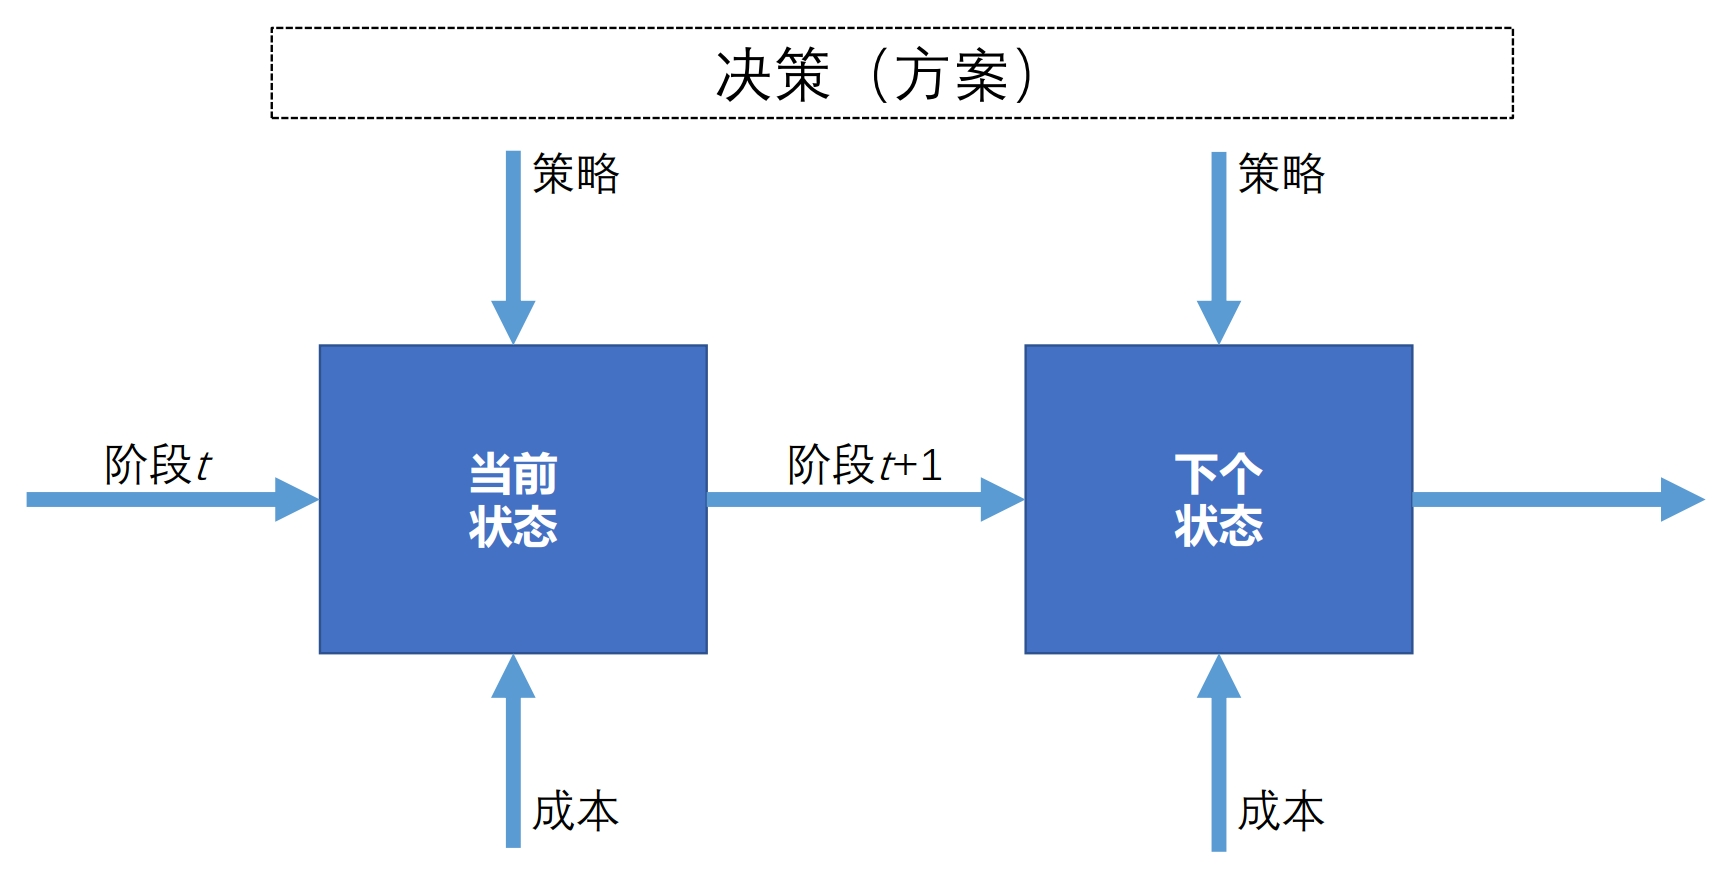
\includegraphics[width=0.8\textwidth]{pic/1.1.1.png}
    \caption{序列决策模型的过程示意}
\end{figure}

用新的符号集表示Markov性即为:

\begin{equation}
    \begin{aligned}
         & P\{S_{t+1}=s_{t+1}|S_t=s_t,A_t=a_t,S_{t-1}=s_{t-1},A_{t-1}\cdots,S_0=s_0\} \\=&P\{S_{t+1}=s_{t+1}|S_t=s_t,A_t=a_t\}
    \end{aligned}
\end{equation}

\subsubsection{Markov决策过程的表示方法}

系统方程:

\begin{equation}
    s_{t+1}=f(s_t,a_t,w_t)
\end{equation}

其中$w_t\in W$为随机扰动,$w_t$的分布与$t$无关,且与$s_t,a_t$无关。$t+1$时刻的状态$s_{t+1}$只与$t$时刻的状态$s_t$和$t$时刻的决策$a_t$有关。

转移概率矩阵:

\begin{equation}
    P_{a}(S_1,S_2)=P\{s_{t+1}=S_2|a_t=S_1,a_t=a\}
\end{equation}

给定当前状态为$s_t$,决策为$a_t$,则下一状态为$s_{t+1}$的概率为$P_{a_t}(s_t,s_{t+1})$。

一个Markov决策过程可以用一个四元组$(S,A,P,g)$来表示。

\begin{example}
    排队网络模型

    假设网络模型包括3台服务器, 2个不同的外部任务入口, 2条固定的工作流程1,2,3和4,5,6,7,8,在不同处理阶段的形成8个排队任务。

    \begin{figure}[ht]
        \centering
        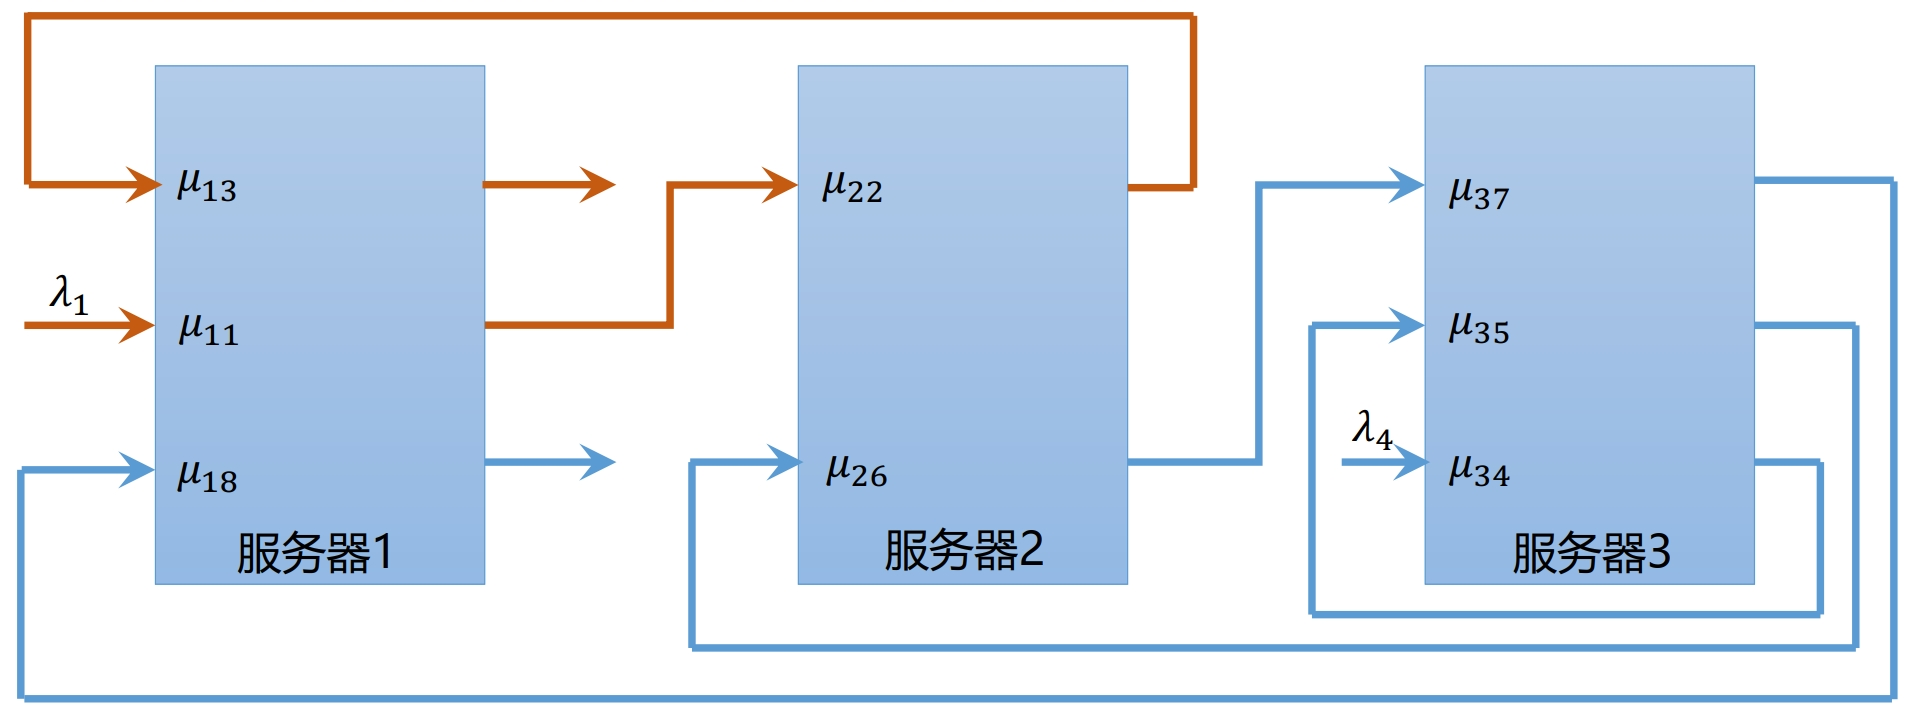
\includegraphics[width=0.8\textwidth]{pic/1.1.2.png}
        \caption{排队网络模型}
    \end{figure}

    我们假设服务时间满足几何随机变量:当服务器 $i$ 在一个时间步内服务于队列 $j$ 中的某一单元时,在本时间步内结束服务的概率为 $\mu _{ij}$,并独立于之前对该单元的服务。

    满足:
    \begin{enumerate}[itemsep=0pt,parsep=0pt]
        \item 任一时间步内,新的工作单元可以概率$\lambda_j$从队列$j=1,4$加入本系统;
        \item 新的工作单位独立于之前到达的工作单元;
        \item 某工作流程完成后, 此工作单元将被移送到整个流程的下一队列;
        \item 当所有流程已完成则该工作单元直接退出系该统。
    \end{enumerate}

    由于每个服务器都服务于多个队列,则在单个时间步内,必须选择确定服务器为哪个队列服务。这种选择可用八维向量代码$\alpha$编码,说明正接受服务的队列,并满足每个服务器只为单个队列服务的条件, 即$\alpha_i \in \{0,1\}$ ,且 $\alpha_1 +\alpha_3 +\alpha_8 \leq  1$,$\alpha_2 + \alpha_6 \leq 1$,$\alpha_4 + \alpha_5 + \alpha_7 \leq 1$。

    我们用对系统$x$的函数$u$来表述这个策略,该策略返回服务器工作分配情况。我们可用转移概率来表示队列的长度的变化——下一状态队列长度$x(t+1)$的条件概率由当前系统状态队列长度$x(t)$和决策$a(t)$确定,例如:

    到达队列1:
    \begin{equation}
        P(x_1(t+1)=x_1(t)+1|x_1(t),a(t))=\lambda_1
    \end{equation}

    离开队列1且到达队列2:
    \begin{equation}
        \begin{aligned}
             & P(x_1(t+1)=x_1(t)-1,x_2(t+1)=x_2(t)+1|x_1(t),x_2(t),a(t)) \\=&\mu_{11}I(x_1(t)>0,a_1(t)=1)
        \end{aligned}
    \end{equation}

    离开队列2且到达队列3:
    \begin{equation}
        \begin{aligned}
             & P(x_2(t+1)=x_2(t)-1,x_3(t+1)=x_3(t)+1|x_2(t),x_3(t),a(t)) \\=&\mu_{22}I(x_2(t)>0,a_2(t)=1)
        \end{aligned}
    \end{equation}

    离开队列3:
    \begin{equation}
        \begin{aligned}
            P(x_3(t+1)=x_3(t)-1|x_3(t),a(t))=\mu_{13}I(x_3(t)>0,a_3(t)=1)
        \end{aligned}
    \end{equation}

    其中$I(\cdot)$为指示函数,表示括号内条件为真时函数值为1,否则为0。


\end{example}

\subsubsection{最优准则}

最优准则——用以定义如何对不同时刻t的成本进行求和。

1. 有限阶段总成本:

\begin{equation}
    E[\sum_{t=0}^{T-1}g_{a_t}(s_t)|s_0=s]
\end{equation}

2. 平均成本:

\begin{equation}
    \lim_{T\rightarrow \infty}E[\frac{1}{T}\sum_{t=0}^{T-1}g_{a_t}(s_t)|s_0=s]
\end{equation}

3. 无限折扣成本:

\begin{equation}
    E[\sum_{t=0}^{\infty}\alpha^tg_{a_t}(s_t)|s_0=s]
\end{equation}

\begin{note}
    $\alpha \in (0,1)$ 是表示即时优先的折扣因子,特别的,当状态矢量空间和行为空间位有限集时, $ \bar{\alpha} < 1$足够大,从而对于所有的$\alpha > \bar{\alpha}$折扣成本问题的最优策略对于平均成本问题也是最优。

    采用折扣因子简化了分析和计算方法:数学表达上的方便、避免产生无限回报的情况、可以体现即时回报比延迟回报优先性。
\end{note}

\section{Markov决策过程的求解方法}

\subsection{有限阶段问题:逆推归纳法}

有限阶段内成本最小的策略,就是求解如下最优化问题:

\begin{equation}
    \min_{u_0,u_1,\cdots,u_{T-1}}E[\sum_{t=0}^{T-1}g_{a_t}(s_t)|s_0=s]
\end{equation}

动态规划的核心思想是:把方程改写成以下方程就可以大大简化寻求最优解的计算:
\begin{equation}
    \min_{a\in A_s}\left\{ g_a(x)+\sum_{s'\in S}P_a(s,s')\min_{u_1,\cdots,u_{T-1}}E[\sum_{t=1}^{T-1}g_{a_t}(s_t)|s_1=s']\right\}
\end{equation}

我们定义代价函数$J(s,t_0)$为从时刻$t_0$到时刻$T$的最优代价,即:
\begin{equation}
    J(s,t_0)=\min_{u_{t_0},\cdots,u_{T-1}}E[\sum_{t=t_0}^{T-1}g_{a_t}(s_t)|s_{t_0}=s]
\end{equation}

则有:
\begin{equation}
    J(s,t_0)=\min_{a\in A_s}\left\{ g_a(x)+\sum_{s'\in S}P_a(s,s')J(s',t_0+1)\right\}
\end{equation}

这是一个递归方程,从$J(s,T)=0$开始,逐步向前递推,直到$J(s,0)$,即可得到最优策略。

\begin{note}
    注意: 找到对应所有的$J(x,t)$需要大量的计算,计算量随着时间和状态的数量增大而线性增长,即使存在大量的呈指数增长的策略。
\end{note}

\begin{example}
    应急救援问题

    某应急救援车需要从$s$地出发到$t$地参与应急救援,期间的道路系统如下图所示,图中的圆圈表示途径的地方,连接两地的箭头表示道路,上面的数字表示该路段长度,箭头表示方向。试求$s$地到$t$地的最佳救援路线。

    \begin{figure}[ht]
        \centering
        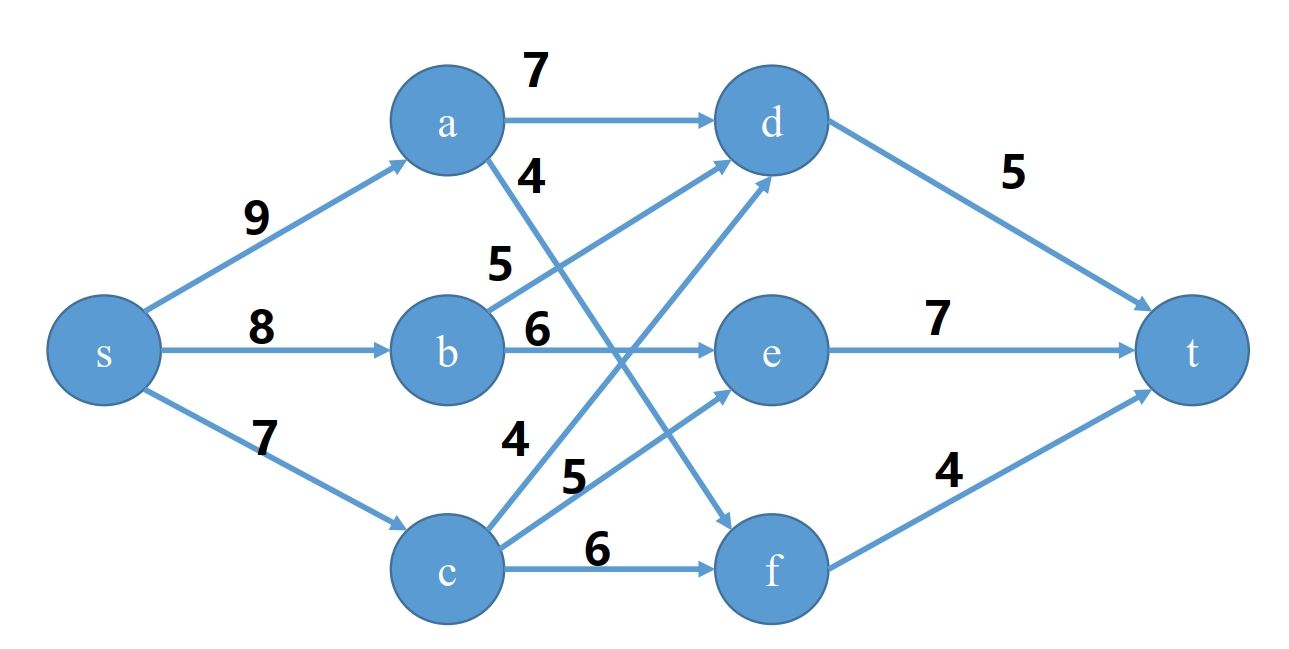
\includegraphics[width=0.8\textwidth]{pic/1.2.1.png}
        \caption{应急救援问题}
    \end{figure}

    \textbf{第一步:划分阶段}

    $k=1, 2, 3$表示三个阶段。

    \textbf{第二步:定义状态变量}

    状态变量$x_k$取为$k$阶段所在地,则有:
    \begin{equation}
        \begin{aligned}
            x_1 \in S_1 & = \{s\}
            x_2 \in S_2 & = \{a,b,c\} \\
            x_3 \in S_3 & = \{d,e,f\} \\
            x_4 \in S_4 & = \{t\}     \\
        \end{aligned}
    \end{equation}

    \textbf{第三步:定义策略和决策集}

    $k$阶段需要确定下一步走向哪里, $u_k(x_k)$即为$k$阶段, 状态为$x_k$时的策略:
    \begin{equation}
        \begin{aligned}
             & u_1 \in U_1 = \{a,b,c\}       \\
             & u_2(a) \in U_2(a) = \{d,f\}   \\
             & u_2(b) \in U_2(b) = \{d,e\}   \\
             & u_2(c) \in U_2(c) = \{d,e,f\} \\
             & u_3 \in U_3 = \{t\}           \\
        \end{aligned}
    \end{equation}

    \textbf{第四步:求解}

    根据有限阶段问题的逆推归纳法,可以逆序地求出条件最优代价函数值集合和条件最优策略集合。

    1.对第3阶段所有可能的状态$S_3 = \{d,e,f\}$ 计算条件最优代价函数值:

    第三阶段末已到达目的地,故$J_4(t) = 0$。
    \begin{equation}
        \begin{aligned}
            J_3(d) = \min_{u_3 \in U_3} \{g_{u_3}(d,t)+J_4(t)\} = 5 \\
            J_3(e) = \min_{u_3 \in U_3} \{g_{u_3}(e,t)+J_4(t)\} = 7 \\
            J_3(f) = \min_{u_3 \in U_3} \{g_{u_3}(f,t)+J_4(t)\} = 4 \\
        \end{aligned}
    \end{equation}
    其中$u_3(d) = u_3(e) = u_3(f) = t$。

    2.对第2阶段所有可能的状态$S_3 = \{a,b,c\}$ 计算条件最优代价函数值:

    \begin{equation}
        \begin{aligned}
            J_2(a) & = \min_{s_3 \in {d,f}} \{g_{u_2(a)}(a,s_3)+J_3(s_3)\}                                                                   \\
                   & =\min\left\{\begin{aligned} g_{u_2}(a,d)+ J_3(d) \\ g_{u_2}(a,f)+ J_3(f) \end{aligned} \right\}                         \\
                   & = \min\left\{\begin{aligned} 7+5 \\ 4+4 \end{aligned} \right\} =8                                                       \\
            J_2(b) & = \min_{s_3 \in {d,e}} \{g_{u_2(b)}(b,s_3)+J_3(s_3)\}                                                                   \\
                   & =\min\left\{\begin{aligned} g_{u_2}(b,d)+ J_3(d) \\ g_{u_2}(b,e)+ J_3(e) \end{aligned} \right\}                         \\
                   & = \min\left\{\begin{aligned} 5+5 \\ 6+7 \end{aligned} \right\} =10                                                      \\
            J_2(c) & = \min_{s_3 \in {d,e,f}} \{g_{u_2(c)}(c,s_3)+J_3(s_3)\}                                                                 \\
                   & =\min\left\{\begin{aligned} g_{u_2}(c,d)+ J_3(d) \\ g_{u_2}(c,e)+ J_3(e) \\ g_{u_2}(c,f)+ J_3(f) \end{aligned} \right\} \\
                   & = \min\left\{\begin{aligned} 4+5 \\ 5+7 \\ 6+4 \end{aligned} \right\} =9                                                \\
        \end{aligned}
    \end{equation}
    其中$u_2(a) = d$,$u_2(b) = d$,$u_2(c) = c$。

    类似求解第一阶段,可以得到$s\rightarrow c\rightarrow d\rightarrow t$:

    \begin{figure}[ht]
        \centering
        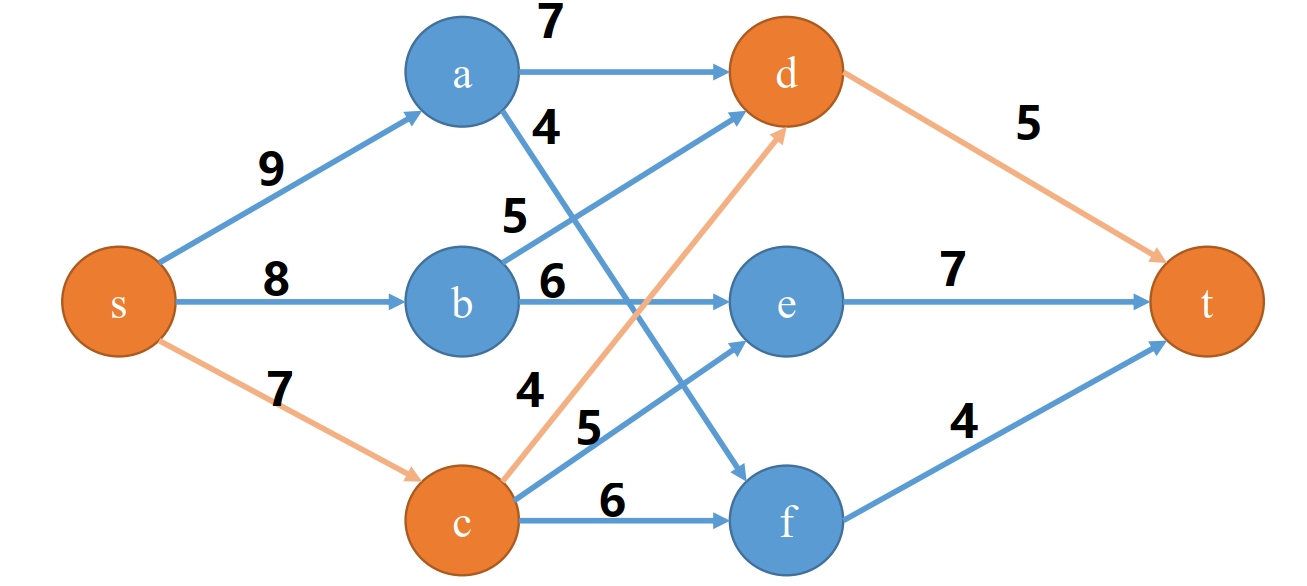
\includegraphics[width=0.8\textwidth]{pic/1.2.2.png}
        \caption{应急救援问题的最优策略}
    \end{figure}

\end{example}

\subsection{折扣成本问题:Bellman方程}

\subsubsection{代价函数与Bellman方程}

同上面的有限阶段问题类似,我们可以定义折扣成本问题的条件最优代价函数值:
\begin{equation}
    J(s,t_0)=\min_{u\in U}E[\sum_{t=t_0}^{\infty}\alpha^{t-t_0}g_{a_t}(s_t)|s_{t_0}=s]
    \label{eq:1.2.1}
\end{equation}

则有:
\begin{equation}
    J(s,t_0)=\min_{a\in A_s}\left\{ g_a(x)+\alpha\sum_{s'\in S}P_a(s,s')J(s',t_0+1)\right\}
\end{equation}

对于无限范围的情况,由\ref{eq:1.2.1}可知,对于任意的$t$和$t'$,总有$J(s,t)=J(s,t')$,即$J(s,t)$与$t$无关,我们可以将其简写为$J(s)$。

这是因为:
\begin{equation}
    \begin{aligned}
        J(s,t) & = \min_{u\in U}E[\sum_{t=t_0}^{\infty}\alpha^{t-t_0}g_{a_t}(s_t)|s_{t_0}=s]    \\
               & = \sum_{t=t_0}^{\infty}\alpha^{t-t_0}P_u(s_{t_0}=s,s_t=\sigma)g_u(s)(\sigma)   \\
               & = \sum_{t=t_0}^{\infty}\alpha^{t-t_0}P_u(s_{t-t_0}=s,s_0=\sigma)g_u(s)(\sigma) \\
               & = \sum_{t=0}^{\infty}\alpha^{t}P_u(s_{t}=s,s_0=\sigma)g_u(s)(\sigma)           \\
    \end{aligned}
\end{equation}
是一个和$t$无关的数。其中$\sigma$为最终状态,转移矩阵与$t$无关。也可以通过无后效性来理解。

同样地$u$也与$t$无关,称为平稳策略。我们给出了Bellman方程的最终形式:

\begin{equation}
    J(s)=\min_{a\in A_s}\left\{ g_a(x)+\alpha\sum_{s'\in S}P_a(s,s')J(s')\right\}
\end{equation}

\subsubsection{动态规划算子}

对于每一个平稳策略$u$,我们用$g_u$表示元项为$g_{u_x}(x)$的矢量,$P_u$表示元项为$P_{u_x}(x)$的矩阵。现在来定义动态规划算子$T$和$T_u$。

我们可以将Bellman方程写成算子的形式:
\begin{equation}
    T_uJ=g_u+\alpha P_uJ
\end{equation}
\begin{equation}
    TJ=\min_{u\in U}T_uJ
\end{equation}
其中$J$是一个向量,记录每一个状态的最优代价函数值。

从而有:
\begin{equation}
    J=TJ
\end{equation}

一般来讲,对于任意函数$J$,若$T_uJ=TJ$ 则认为策略$u$是与$J$强相关。我们把与$J$强相关的策略记为$u_J$,即$u_J$是$T_uJ=TJ$的解。

\begin{note}
    例如$T_{u_{J_{u_{k}}}}$。

    $u_{k}$: 可选行为集中的某一策略;

    $J_{u_{k}}$: 以$u_{k}$为策略时的代价函数;

    $u_{J_{u_{k}}}$: 以$u_{k}$强相关的策略;

    $T_{u_{J_{u_{k}}}}$: 以$u_{J_{u_{k}}}$为策略时的动态规划算子。
\end{note}

动态规划算子的三大特性: 单调性、 偏移性、 最大模收缩

\begin{enumerate}[itemsep=0pt,parsep=0pt]
    \item 单调性: 若$J_1\leq J_2$,则$TJ_1\leq TJ_2$。
    \item 偏移性: 对于所有的$J$和属于R的常数$c$,有$T(J+ce)=TJ+\alpha ce$。
    \item 最大模收缩: $\|TJ_1-TJ_2\|_{\infty}\leq \alpha \|J_1-J_2\|_{\infty}$。
\end{enumerate}

证明:

1. 单调性:

\begin{equation}
    \begin{aligned}
        TJ_1\leq T_{u_{J_2}}J_1 & = g_{u_{J_2}}+\alpha P_{u_{J_2}}J_1    \\
                                & \leq g_{u_{J_2}}+\alpha P_{u_{J_2}}J_2 \\
                                & = T_{u_{J_2}}J_2                       \\
                                & \leq TJ_2                              \\
    \end{aligned}
\end{equation}

2. 偏移性:

\begin{equation}
    \begin{aligned}
        T(J+ce) & = \min_{u\in U}T_u(J+ce)          \\
                & = \min_{u\in U}T_uJ+\alpha cP_u e \\
                & = TJ+\alpha ce                    \\
    \end{aligned}
\end{equation}

3. 最大模收缩:


注意到:
\begin{equation}
    \begin{aligned}
        J = J + J' - J' \leq J' + \|J-J'\|_{\infty}e
    \end{aligned}
\end{equation}


\begin{equation}
    \begin{aligned}
        TJ - TJ'            & = T(J-J')                            \\
                            & \leq T(J' + \|J-J'\|_{\infty}e - J') \\
                            & = \alpha \|J-J'\|_{\infty}e          \\
        \|TJ-TJ'\|_{\infty} & \leq \alpha \|J-J'\|_{\infty}
    \end{aligned}
\end{equation}
其中用到了前两条性质。

\subsection{数值迭代方法}

\subsubsection{Bellman方程解的唯一性}

对于Bellman方程,我们可以通过迭代的方法求解。我们可以从任意的$J_0$开始,通过$J_{k+1}=TJ_k$来迭代求解。

我们先证明Bellman方程的解的存在唯一性。

\begin{proof}
    1. 存在性:

    由于$T$是一个压缩映射,所以$T$有唯一不动点,即$TJ=J$有唯一解$J^*$。

    2. 唯一性:

    假设$J_1$和$J_2$都是Bellman方程的解,则有:
    \begin{equation}
        \begin{aligned}
            J_1 & = T J_1 \\
            J_2 & = T J_2 \\
        \end{aligned}
    \end{equation}

    从而有:
    \begin{equation}
        \begin{aligned}
            \|J_1-J_2\|_{\infty} & = \|TJ_1-TJ_2\|_{\infty}         \\
                                 & \leq \alpha \|J_1-J_2\|_{\infty}
        \end{aligned}
    \end{equation}

    由于$\alpha < 1$,所以$J_1=J_2$。
\end{proof}

这就说明数值迭代方法是收敛的,一定可以找到Bellman方程的解。而且解是唯一的。

\begin{example}

    段数不定的最短路线问题(不定期决策过程)

    $n$个点相互连接组成 一个连通图(图中$n=5$),各点标号为$1,2,…, n$ 。任意两点$i,j$之间的距离(费用)记作$d_{ij}$ 。求任意一点$i$到点$n$(靶点)的最短路线(距离)。

    \begin{figure}[ht]
        \centering
        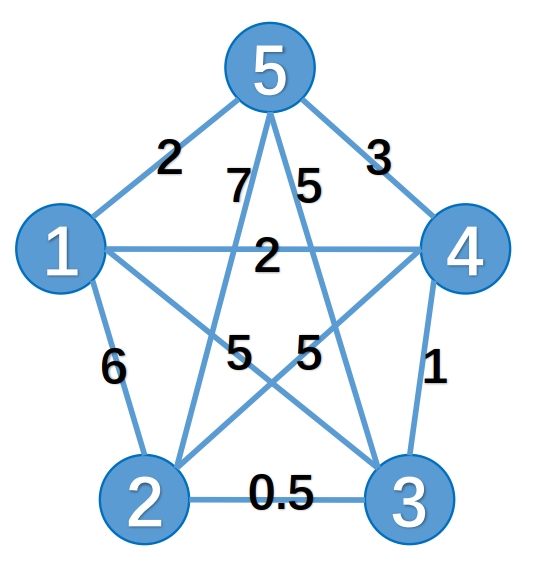
\includegraphics[width=0.4\textwidth]{pic/1.2.3.png}
        \caption{段数不定的最短路线问题}
    \end{figure}

    1.从$i$点走一步到靶点5的最优距离为$J_1(i)$ , 则显然有:
    \begin{equation}
        J_1(i)=d_{i5}
    \end{equation}
    具体说:
    \begin{equation}
        \begin{aligned}
            J_1(1) & = d_{15} = 2 \\
            J_1(2) & = d_{25} = 7 \\
            J_1(3) & = d_{35} = 5 \\
            J_1(4) & = d_{45} = 3 \\
            J1(5)  & = d_{55} = 0 \\
        \end{aligned}
    \end{equation}

    其中最优决策为:
    \begin{equation}
        u_1(i)=\arg \min_{j\in N(i)}\{d_{ij}\}
    \end{equation}
    具体说:
    \begin{equation}
        \begin{aligned}
            u_1(1) & = 5 \\
            u_1(2) & = 5 \\
            u_1(3) & = 5 \\
            u_1(4) & = 5 \\
            u_1(5) & = 5 \\
        \end{aligned}
    \end{equation}

    2.从$i$点走两步到靶点5的最优距离为为$J_2(i)$ , 根据最优化原理得:

    \begin{equation}
        J_2(i)=\min_{j\in N(i)}\{d_{ij}+J_1(j)\}
    \end{equation}
    具体说:
    \begin{equation}
        \begin{aligned}
            J_2(1) & = \min\{d_{11}+J_1(1),d_{12}+J_1(2),d_{13}+J_1(3),d_{14}+J_1(4),d_{15}+J_1(5)\} \\
                   & = \min\{0+2,6+7,5+5,2+3,2+0\}                                                   \\
                   & = 2                                                                             \\
            J_2(2) & = \min\{d_{21}+J_1(1),d_{22}+J_1(2),d_{23}+J_1(3),d_{24}+J_1(4),d_{25}+J_1(5)\} \\
                   & = \min\{6+2,0+7,0.5+5,5+3,7+0\}                                                 \\
                   & = 5.5                                                                           \\
            J_2(3) & = \min\{d_{31}+J_1(1),d_{32}+J_1(2),d_{33}+J_1(3),d_{34}+J_1(4),d_{35}+J_1(5)\} \\
                   & = \min\{5+2,0.5+7,0+5,1+3,5+0\}                                                 \\
                   & = 3                                                                             \\
            J_2(4) & = \min\{d_{41}+J_1(1),d_{42}+J_1(2),d_{43}+J_1(3),d_{44}+J_1(4),d_{45}+J_1(5)\} \\
                   & = \min\{2+2,5+7,1+5,0+3,3+0\}                                                   \\
                   & = 3                                                                             \\
            J_2(5) & = \min\{d_{51}+J_1(1),d_{52}+J_1(2),d_{53}+J_1(3),d_{54}+J_1(4),d
            _{55}+J_1(5)\}                                                                           \\
                   & = 0                                                                             \\
        \end{aligned}
    \end{equation}

    其中最优决策为:
    \begin{equation}
        u_2(i)=\arg \min_{j\in N(i)}\{d_{ij}+J_1(j)\}
    \end{equation}
    具体说:
    \begin{equation}
        \begin{aligned}
            u_2(1) & = 5 \\
            u_2(2) & = 3 \\
            u_2(3) & = 4 \\
            u_2(4) & = 5 \\
            u_2(5) & = 5 \\
        \end{aligned}
    \end{equation}

    3.从$i$点走三步到靶点5的最优距离为为$J_3(i)$ , 根据最优化原理得:

    按照同样的方法解得:
    \begin{equation}
        \begin{aligned}
            J_3(1) & = 2   \\
            J_3(2) & = 4.5 \\
            J_3(3) & = 4   \\
            J_3(4) & = 3   \\
            J_3(5) & = 0   \\
        \end{aligned}
    \end{equation}
    \begin{equation}
        \begin{aligned}
            u_3(1) & = 5 \\
            u_3(2) & = 3 \\
            u_3(3) & = 4 \\
            u_3(4) & = 5 \\
            u_3(5) & = 5 \\
        \end{aligned}
    \end{equation}

    4.从$i$点走四步到靶点5的最优距离为为$J_4(i)$ , 根据最优化原理得:

    按照同样的方法解得:
    \begin{equation}
        \begin{aligned}
            J_4(1) & = 2   \\
            J_4(2) & = 4.5 \\
            J_4(3) & = 4   \\
            J_4(4) & = 3   \\
            J_4(5) & = 0   \\
        \end{aligned}
    \end{equation}
    \begin{equation}
        \begin{aligned}
            u_4(1) & = 5 \\
            u_4(2) & = 3 \\
            u_4(3) & = 4 \\
            u_4(4) & = 5 \\
            u_4(5) & = 5 \\
        \end{aligned}
    \end{equation}
    数值稳定,说明迭代完成。

    下面是示例代码:

\end{example}

\begin{lstlisting}[language=python]
import numpy as np

def compute_shortest_paths(n, distances):
"""
计算最短路径的函数。

参数:
n -- 点的个数
distances -- 二维数组,表示每两点之间的距离

返回:
J -- 每个点到目标点的最短路径长度
u -- 每个点到目标点的最优决策路径
"""
# 初始化J和u数组。J记录最短路径长度,u记录最优决策路径。
J = np.zeros((n, n))
u = np.zeros((n, n), dtype=int)

# 初始条件:从每个点到目标点n的直接距离
for i in range(n):
J[i][0] = distances[i][n-1]
u[i][0] = n

# 进行k步迭代,计算每个点通过k步到达目标点的最短路径
for k in range(1, n):
for i in range(n):
# 计算通过中间点到达目标点的最短距离
min_distance = float('inf')
for j in range(n):
distance = distances[i][j] + J[j][k-1]
if distance < min_distance:
min_distance = distance
u[i][k] = j + 1  # 存储最优决策点
J[i][k] = min_distance

return J, u

# 假设的距离矩阵,这里需要具体的距离数据来填充
n = 5  # 点的数量
distances = np.array([
        [0, 6, 5, 2, 2],
        [6, 0, 0.5, 5, 7],
        [5, 0.5, 0, 1, 5],
        [2, 5, 1, 0, 3],
        [2, 7, 5, 3, 0]
    ])

# 计算最短路径
J, u = compute_shortest_paths(n, distances)
\end{lstlisting}

\subsubsection{Gauss-Seidel迭代}

\href{https://en.wikipedia.org/wiki/Gauss%E2%80%93Seidel_method}{Gauss-Seidel迭代}是一种特殊的数值迭代方法,它的特点是每次迭代都是在实时更新的结果上进行的,而不是像一般的迭代方法那样,每次迭代都是在上一次迭代的结果上进行的。

不同于上面的Jacobi迭代,Gauss-Seidel迭代是一种逐点更新的方法,即每次更新一个点,而不是一次更新所有点。这样的好处是可以节省内存,因为每次只需要存储一个点的值,而不是所有点的值。

如果$A=D+L+U$,其中$D$是$A$的对角矩阵,$L$是$A$的严格下三角矩阵,$U$是$A$的严格上三角矩阵,则普通的Jacobi迭代可以写成:
\begin{equation}
    Dx^{(k+1)}=b-(L+U)x^{(k)}
\end{equation}
其中$x^{(k)}$是第$k$次迭代的结果,$b$是方程组$Ax=b$的右端项。

如果我们写出$Ax=b$的每一行,第$i$行为:
\begin{equation}
    \sum_{j=1}^{n}a_{ij}x_j=b_i
\end{equation}

对这一行的求解为:
\begin{equation}
    x_i^{({\color{red}k+1})}=\frac{1}{a_{ii}}(b_i-\sum_{j=1}^{i-1}a_{ij}x_j^{({\color{red}k})}-\sum_{j=i+1}^{n}a_{ij}x_j^{({\color{red}k})})
\end{equation}

如果$A=D+L+U$,其中$D$是$A$的对角矩阵,$L$是$A$的严格下三角矩阵,$U$是$A$的严格上三角矩阵,则Gauss-Seidel迭代可以写成:
\begin{equation}
    (D+K)x^{(k+1)}=b-Ux^{(k)}
\end{equation}

对应的迭代形式为:
\begin{equation}
    x_i^{({\color{red}k+1})}=\frac{1}{a_{ii}}(b_i-\sum_{j=1}^{i-1}a_{ij}x_j^{({\color{red}k+1})}-\sum_{j=i+1}^{n}a_{ij}x_j^{({\color{red}k})})
\end{equation}

Jacobi 迭代和 Gauss-Seidel 迭代形式几乎一样。但 Gauss-Seidel 及时利用了最新的迭代结果,直观上比 Jacobi 效率更高。\footnote{这一段论述来源于\href{https://zhuanlan.zhihu.com/p/389389672}{知乎},其中给出了很详细的解释和图示。}

我们可以定义新的算符:

\begin{equation}
    FJ(x)=\min_{u\in U}\left\{ g_u(x)+\alpha\sum_{y<x}P_u(x,y)FJ(y)+\alpha \sum_{y\geq x}P_U(x,y)J(y)\right\}
\end{equation}

同样地,这样的算符也是压缩映射,不动点也为Bellman方程的解$J^*$。

\subsection{平稳策略的最优化}

从一个引理出发:

\begin{quotation}

    如果$J\leq TJ$,则$J\leq J^*$; 如果$J\geq TJ$,则$J\geq J^*$。其中$J^*$为Bellman方程的解。

\end{quotation}


该引理利用迭代显然。

而对于平稳策略,就有以下的性质:

\begin{quotation}

    $u\in U$表示任意策略,$u^*=u_{J^*}$是最优策略(有$J^*=TJ^*=T_{u^*}J^*$),则有:$J_u\geq J_{u^*}=J^*$。如果$u$为满足$T_uJ^*\neq TJ^*$的任意策略,则至少存在一个状态$x$,使得$J_u(x)>J^*(x)$。

\end{quotation}

\begin{proof}
    先说明$J_{u^*}=J^*$。

    由于$J^*=TJ^*=T_{u^*}J^*$,所以$J^*$是$T_{u^*}$的不动点,而$T_{u^*}$是压缩映射,所以$J^*$是唯一的不动点,即$J_{u^*}=J^*$。

    对于其他任何策略,都有$J_u\geq TJ_u$,所以$J_u\geq TJ_u\geq TJ^*=J^*$。

    考虑平稳策略$u$,如果$T_uJ^*\neq TJ^*$,即$T_uJ^*\geq TJ^*$,并存在至少一个状态$x$,使得$T_uJ^*(x)>TJ^*(x)$,则有:
    \begin{equation}
        \begin{aligned}
            J_u(x) & \geq T_uJ^*(x) > TJ^*(x) = J^*(x)
        \end{aligned}
    \end{equation}
\end{proof}

\begin{example}
    折扣成本相关例题分析:

    某地A发生了一场地震,为了尽快进行灾后救援,政府需要从灾区外某地B向灾区运送救援物资,而地震后五天内的救援是十分重要的。因此,我们模拟一个向震区运送物资的情景,并考虑如何在五天内运送尽可能多的物资。

    假设从B地前往A地的道路大多被地震破坏封堵,眼下还有两条路径,分别标记为M和N, B地一共有$1000$辆汽车可用于物资运输,并且通过M、 N路径前往A地往返一次都只需要一天的时间。M路受地震影响较小,路况较好,汽车往返一次不发生故障的概率$\beta= 0.9$, 但是M路需要通过一座受过地震影响的桥梁,为了保障桥梁的安全, M路上的汽车载重不能超过$5$吨。N路不需要通过这样的桥梁,汽车可以满载$8$吨,但是由于N路受地震影响较大,路况较差,往返一次后车辆不发生故障的概率$\alpha = 0.7$。

    在这紧张的五天内,每天晚上都会对所有的汽车进行检修, 若没有发生故障可以将汽车状态恢复如初;一旦发生故障,简单的检修不足以让该车辆在五天内恢复正常工作.假设发生故障的汽车可以顺利完成本次运输任务并成功返回B地。

    显然,分配不同数目的车辆分别从M、 N两条路同时向灾区运送物资才能在五天内运送更多的物资,而如何分配两条路上车辆的比例则是我们需要解决的问题。

    \textbf{问题分析}

    从假设中可以看出,五天内的分配策略之间是无后效性的,可以考虑用Markov决策过程进行分析。

    首先对此过程进行一些假设:

    设阶段$k$表示天数,则$k = 1,2,3,4,5$;状态变量$S_k$表示第$k$天初所拥有的未发生故障的车辆数目,亦即$k-1$天晚上未发生故障的车辆数目;决策变量$x_k$表示在第$k$天分配从N路前往灾区的车辆数目,同时得到$S_k-x_k$为当日分配从M路前往灾区的车辆数目。

    可得状态转移方程为:
    \begin{equation}
        S_{k+1} = \alpha x_k+\beta(S_k-x_k) = 0.9S_k-0.2x_k
    \end{equation}

    允许决策的集合为:
    \begin{equation}
        U_k = \{x_k\in \mathbb{N} | 0\leq x_k\leq S_k\}
    \end{equation}

    设一个阶段指标$g_k(S_k, x_k)$作为每个阶段向灾区运送的物资总和:
    \begin{equation}
        g_k(S_k, x_k) = 8x_k+5(S_k-x_k) = 5S_k+3x_k
    \end{equation}

    设有最优函数$J_k(S_k)$表示从现有的资源$S_k$出发,采取最优策略向灾区运送的物资总量,可以得到Bellman方程:
    \begin{equation}
        \begin{aligned}
            J_k(S_k) & = \max_{x_k\in U_k}\{g_k(S_k, x_k)+ J_{k+1}(S_{k+1})\}  \\
                     & = \max_{x_k\in U_k}\{5S_k+3x_k+J_{k+1}(0.9S_k-0.2x_k)\}
        \end{aligned}
    \end{equation}
    对于边界情况我们有: $J_6(S_6) = 0$。

    在$k= 5$时:
    \begin{equation}
        \begin{aligned}
            J_5(S_5) & = \max_{x_5\in U_5}\{5S_5+3x_5+J_6(S_6)\} \\
                     & = \max_{x_5\in U_5}\{5S_5+3x_5\}
        \end{aligned}
    \end{equation}
    是关于$S_5$的线性函数,其最优策略为$x_5^* = S_5$,最优值为$J_5^*(S_5) = 8S_5$。

    在$k= 4$时:
    \begin{equation}
        \begin{aligned}
            J_4(S_4) & = \max_{x_4\in U_4}\{5S_4+3x_4+J_5(0.9S_4-0.2x_4)\} \\
                     & = \max_{x_4\in U_4}\{5S_4+3x_4+8(0.9S_4-0.2x_4)\}   \\
                     & = \max_{x_4\in U_4}\{12.2S_4+1.4x_4\}
        \end{aligned}
    \end{equation}
    是关于$S_4$的线性函数,其最优策略为$x_4^* = S_4$,最优值为$J_4^*(S_4) = 13.6S_4$。

    以此类推,可以得到:

    $k= 3$时,$J_3^*(S_3) = 17.5S_3$,$x_3^* = S_3$;

    $k= 2$时,$J_2^*(S_2) = 20.8S_2$,$x_2^* = 0$;

    $k= 1$时,$J_1^*(S_1) = 23.7S_1$,$x_1^* = 0$。

    计算结果表明,最优策略为前两天将车辆全部安排从M路走,后三天将全部车辆安排从N路行驶,这样可以实现$5$天内运输的物资数目最大,最大的运量为$23700$吨。由此也可以根据最优策略得出每个阶段的状态,我们可以据此阶段顺序来分别计算每天完好车辆数量:
    \begin{equation}
        \begin{aligned}
            S_1 & = 1000                \\
            S_2 & = 0.9S_1-0.2x_1 = 900 \\
            S_3 & = 0.9S_2-0.2x_2 = 810 \\
            S_4 & = 0.9S_3-0.2x_3 = 567 \\
            S_5 & = 0.9S_4-0.2x_4 = 397 \\
            S_6 & = 0.9S_5-0.2x_5 = 278 \\
        \end{aligned}
    \end{equation}

\end{example}


\subsection{策略迭代}

策略迭代算法过程如下:

\begin{enumerate}[itemsep=0pt,parsep=0pt]
    \item 以策略$u_0$,$k=0$开始;
    \item 代价评估阶段:计算$J_{u_k} = g_{u_k}+\alpha P_{u_k}J_{u_k}$;
    \item 策略改善阶段:选择$u_{k+1} = u_{J_{u_k}}$;
    \item 如果$u_{k+1} = u_k$,则停止,否则令$k=k+1$,转到步骤2。
\end{enumerate}

\begin{note}
    步骤2是为每一次迭代获得更佳的策略。由于策略集是有限的,该算法将在有限的时间步内终止,我们通常用下述定理正式阐述这种概念。
\end{note}

\begin{quote}
    经过有限次迭代后,策略迭代收敛于$u^*$,即$u_k=u^*$,并且$J_{u_k}=J^*$。
\end{quote}

\begin{proof}
    若$u_k$是最优的,即得证。

    否则,存在一个状态$x$,使得$T J_{u_k} <= T_{u_k}J_{u_k} < J_{u_k}$。

    由于$T_{u_{k+1}}J_{u_k} = T_{u_{J_{u_k}}}J_{u_k} = TJ_{u_k}$,且$J_{u_k}=T_{u_k}J_{u_k}$,所以$J_{u_k} = T_{u_{k}}J_{u_k} >= TJ_{u_k} = T_{u_{k+1}}J_{u_k} >= T^n_{u_{k+1}}J_{u_k} \rightarrow J_{u_{k+1}}$。

    因此,策略$u_{k+1}$比策略$u_k$更优,与假设矛盾。
\end{proof}

对于数值迭代步骤:

\begin{enumerate}[itemsep=0pt,parsep=0pt]
    \item $J_0, k = 0$;
    \item $J_{k+1} = T J_k, k = k+1$;
    \item 若$J_{k+1} - J_k < \epsilon$,迭代结束,否则返回步骤2。
\end{enumerate}

数值迭代法和策略迭代法中, 序列$J_j$和$u_k$的收敛性在相当广泛的条件下是可以保证的,一般来说它与状态$S$、 决策$A_{x_t}$ 、状态转移概率 $P_a(x,y)$等的具体形式有关。

\textbf{数值迭代法}的基本思想是:以步数(段数)作为参数,以代价函数作为参考值,先求在各个不同步数下的最优策略,然后从这些最优解中再选出最优者,从而同时确定了最优步数。

\textbf{策略迭代法}的基本思想是:先选定一初始策略$u_0$, 然后按某种方式求得新策略,直至最终求出最优策略。若对某一$k$, 对所有阶段有: $u_{k+1}=u_k$,则称策略收敛,此时, 策略$u_k$就是最优策略。

下面用策略迭代方法重新求解上面的问题:

\begin{example}

    段数不定的最短路线问题(不定期决策过程)

    $n$个点相互连接组成 一个连通图(图中$n=5$),各点标号为$1,2,…, n$ 。任意两点$i,j$之间的距离(费用)记作$d_{ij}$ 。求任意一点$i$到点$n$(靶点)的最短路线(距离)。

    \begin{figure}[ht]
        \centering
        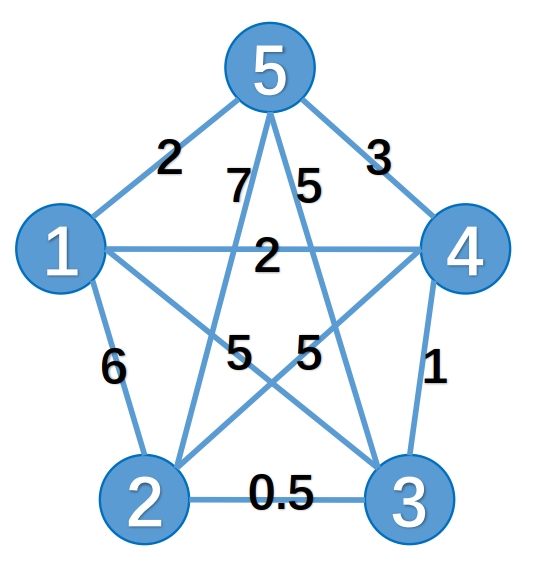
\includegraphics[width=0.4\textwidth]{pic/1.2.3.png}
        \caption{段数不定的最短路线问题}
    \end{figure}

    \textbf{第一步}

    \textbf{1.}

    先选取初始策略$u_1(i)$,例如取$u_1(1)=5,u_1(2)=4,u_1(3)=5,u_1(4)=3$,即$U_1=\{5,4,5,3\}$。注意必须无回路,每点可达靶点。

    \textbf{2.}

    由$u_1$可得$J_1(i)$,由策略迭代法可得:
    \begin{equation}
        \begin{aligned}
            J_1(i) & = d_{i,u_1(i)}+J_1(u_1(i)) \\
            J_1(5) & = 0
        \end{aligned}
    \end{equation}
    由于策略$u_1(1)$和$u_1(3)$直达靶点,应先计算:
    \begin{equation}
        \begin{aligned}
            J_1(1) & = d_{15}+J_1(5) = 2  \\
            J_1(3) & = d_{35}+J_1(5) = 5  \\
            J_1(4) & = d_{43}+J_1(3) = 6  \\
            J_1(2) & = d_{24}+J_1(4) = 11 \\
        \end{aligned}
    \end{equation}

    \textbf{3.}

    由$J_1(i)$可得$u_2(i)$,继续策略迭代。由$\min_{u(i)}[d_{i,u(i)}+J_1(u(i))]$求解$u_2(i)$,可得:

    $u_1(i) = 1$时,
    \begin{equation}
        \min_{u(i)}[d_{i,u(i)}+J_1(u(i))] = \min \begin{bmatrix}
            d_{11}+J_1(1) \\
            d_{12}+J_1(2) \\
            d_{13}+J_1(3) \\
            d_{14}+J_1(4) \\
            d_{15}+J_1(5) \\
        \end{bmatrix} = \min \begin{bmatrix}
            0+2  \\
            6+11 \\
            5+5  \\
            2+6  \\
            2+0  \\
        \end{bmatrix} = 2
    \end{equation}
    从而$u_2(1)=5$,(不在含$d_{ii}$的项取最小值)。

    $u_1(i) = 2$时,
    \begin{equation}
        \min_{u(i)}[d_{i,u(i)}+J_1(u(i))] = \min \begin{bmatrix}
            d_{21}+J_1(1) \\
            d_{22}+J_1(2) \\
            d_{23}+J_1(3) \\
            d_{24}+J_1(4) \\
            d_{25}+J_1(5) \\
        \end{bmatrix} = \min \begin{bmatrix}
            6+2   \\
            0+11  \\
            0.5+5 \\
            5+6   \\
            7+0   \\
        \end{bmatrix} = 5.5
    \end{equation}
    从而$u_2(2)=3$。

    同理可以求得$u_2(3)=5$,$u_2(4)=5$。

    于是第一次策略迭代的结果是:$U_2=\{5,3,5,5\}$。

    \textbf{第二步}

    \textbf{1.}
    以$u_2(i)$为初始策略继续反复使用策略迭代$2$和$3$进行迭代

    \textbf{2.}
    由$u_2$可得$J_2(i)$,由策略迭代法可得:
    \begin{equation}
        \begin{aligned}
            J_2(1) & = d_{15}+J_2(5) = 2   \\
            J_2(3) & = d_{35}+J_2(5) = 5   \\
            J_2(4) & = d_{45}+J_2(5) = 3   \\
            J_2(2) & = d_{23}+J_2(3) = 5.5 \\
        \end{aligned}
    \end{equation}

    \textbf{3.}
    由$J_2(i)$可得$u_3(i)$,继续策略迭代。由$\min_{u(i)}[d_{i,u(i)}+J_2(u(i))]$求解$u_3(i)$,可得:
    \begin{equation}
        \begin{aligned}
            u_3(1) & = 5 \\
            u_3(3) & = 3 \\
            u_3(4) & = 4 \\
            u_3(2) & = 5 \\
        \end{aligned}
    \end{equation}

    于是第二次策略迭代的结果是:$U_3=\{5,3,4,5\}$。

    \textbf{第三步}

    同理迭代得到:$U_4=\{5,3,4,5\}$。

    \textbf{第四步}

    将上面的结果记录下来

    \begin{table}[h]
        \centering
        \setlength{\tabcolsep}{5mm}
        \begin{tabular}{ccccc}
            \toprule
            i        & 1 & 2   & 3 & 4 \\
            \midrule
            $u_1(i)$ & 5 & 4   & 5 & 3 \\
            $J_1(i)$ & 2 & 11  & 5 & 6 \\
            $u_2(i)$ & 5 & 3   & 5 & 5 \\
            $J_2(i)$ & 2 & 5.5 & 5 & 3 \\
            $u_3(i)$ & 5 & 3   & 4 & 5 \\
            $J_3(i)$ & 2 & 4.5 & 5 & 3 \\
            $u_4(i)$ & 5 & 3   & 4 & 5 \\
            \bottomrule
        \end{tabular}
        \caption{策略迭代法结果记录表}
    \end{table}

    从而最优策略为:$u^*=\{5,3,4,5\}$,最优值为$J^*=\{2,4.5,5,3\}$。
\end{example}

\begin{note}
    1. 策略迭代在代价评估阶段,每迭代一次都需要保证每个状态的代价函数收敛,这是非常耗时的; 而数值迭代是采用动态规划的思想来收敛每个状态的代价函数的。

    2. 策略迭代第二步代价评估与数值迭代的第二步十分相似,除了后者用了min操作,前者没有min。因此后者可以得出最有代价函数, 而前者不能得到最有代价。

    3. 策略迭代的收敛速度更快一些,在状态空间较小时,最好选用策略迭代方法。当状态空间较大时,数值迭代的计算量更小一些。

    4. 侧重点不同:策略迭代最后是策略收敛,而值迭代是值函数收敛。

    5. 收敛方式不同:策略迭代是argmin, 而数值迭代是min。
\end{note}

\begin{example}
    状态空间$S=\{1,2\}$ 在状态$1$和状态$2$的可用行动集为$A_1 =
        A_2 = \{m,n\} $. 折扣因子为$\alpha = 0.9$。相应的转移概率和成本函数如下表所示。求最优策略和最大收益。

    \begin{figure}[h]
        \centering 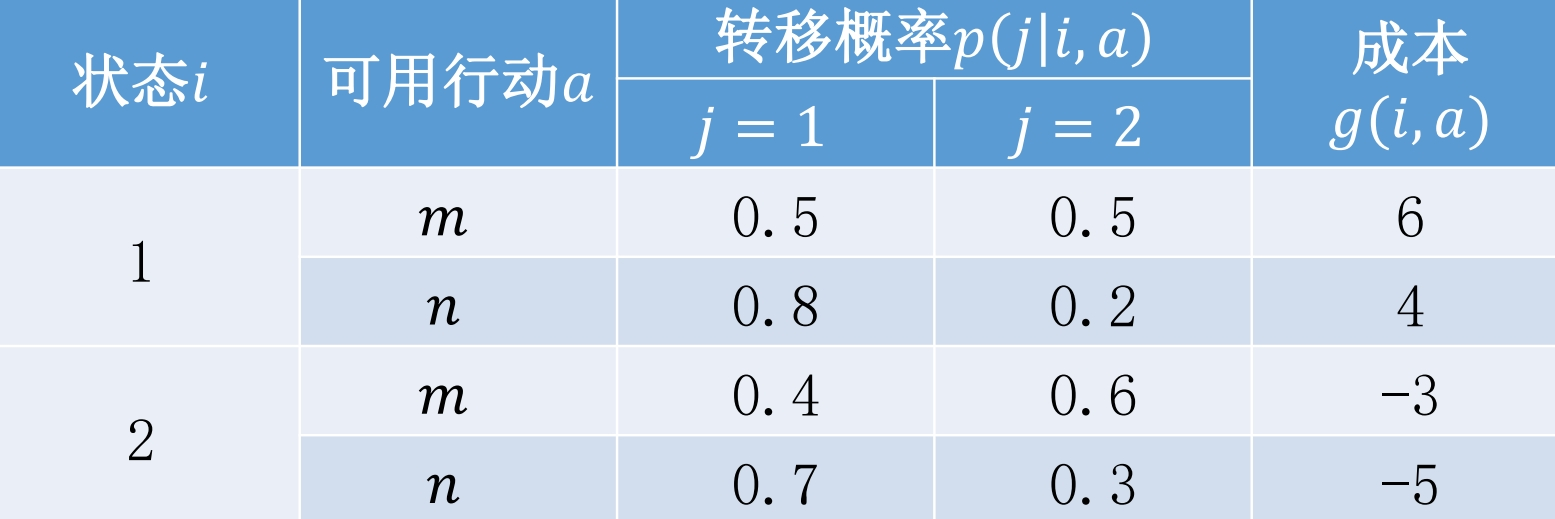
\includegraphics[scale=0.15]{pic/1.3.1.png}
        \caption{状态转移概率和成本函数}
    \end{figure}

    这时由4个平稳策略:
    \begin{equation}
        \begin{aligned}
            u_1 & = \{m,m\} \\
            u_2 & = \{m,n\} \\
            u_3 & = \{n,m\} \\
            u_4 & = \{n,n\} \\
        \end{aligned}
    \end{equation}

    先选择一个初始策略$u_1$,计算$J_1$:
    \begin{equation}
        \begin{aligned}
            6 + 0.9(0.5J_1 + 0.5J_2)  & = J_1 \\
            -3 + 0.9(0.4J_1 + 0.6J_2) & = J_2 \\
        \end{aligned}
    \end{equation}
    解的结果为$J_1(u_1) = 15.49 , J_2(u_1) = 5.60$。

    策略改善:对于状态$1$
    \begin{equation}
        \max \{g(1,a) + 0.9 \sum_{s\in S}p(j|1,a) J_s(u_1)\} = \max \begin{bmatrix}
            0.9(0.5J_1+0.5J_2) + 6 \\
            0.9(0.4J_1+0.6J_2) +4  \\
        \end{bmatrix} = 16.16
    \end{equation}
    采取行为$n$更优。

    对于状态$2$
    \begin{equation}
        \max \{g(2,a) + 0.9 \sum_{s\in S}p(j|2,a) J_s(u_1)\} = \max \begin{bmatrix}
            0.9(0.4J_1+0.6J_2) - 3 \\
            0.9(0.7J_1+0.3J_2) - 5 \\
        \end{bmatrix} = 6.27
    \end{equation}
    采取行为$n$更优。

    改进后的策略为$u_4 = \{n,n\}$。

    继续迭代还是收敛到$u_4$,最优值为$(22.20,12.31)$。
\end{example}

策略迭代的步骤2求解时将需要大量的计算,而异步策略迭代则可以避免这种情况。

其算法如下:

\begin{enumerate}[itemsep=0pt,parsep=0pt]
    \item 以策略$u_0$,$k=0$开始;
    \item 对于子集$s_k\in S$, 执行下面两步骤之一:
          \begin{enumerate}[itemsep=0pt,parsep=0pt]
              \item 数值更新:计算$J_{k+1} = T_{u_k}J_k$;
              \item 策略更新:选择$u_{k+1} = u_{J_{u_k}}$;
          \end{enumerate}
    \item 如果$u_{k+1} = u_k$,则停止,否则令$k=k+1$,转到步骤2。
\end{enumerate}



\chapter{数据驱动的风险量化分析与建模}

数据驱动的风险量化分析与建模是指
\begin{enumerate}[itemsep=0pt,parsep=0pt]
    \item 基于历史灾害数据,通过学习统计分析等多因素分析方法;
    \item 实现对环境、社会等多种因素致灾风险的定量评估;
    \item 构建相应风险评估模型,为决策制定提供数据基础。
\end{enumerate}

\begin{figure}[ht]
    \centering
    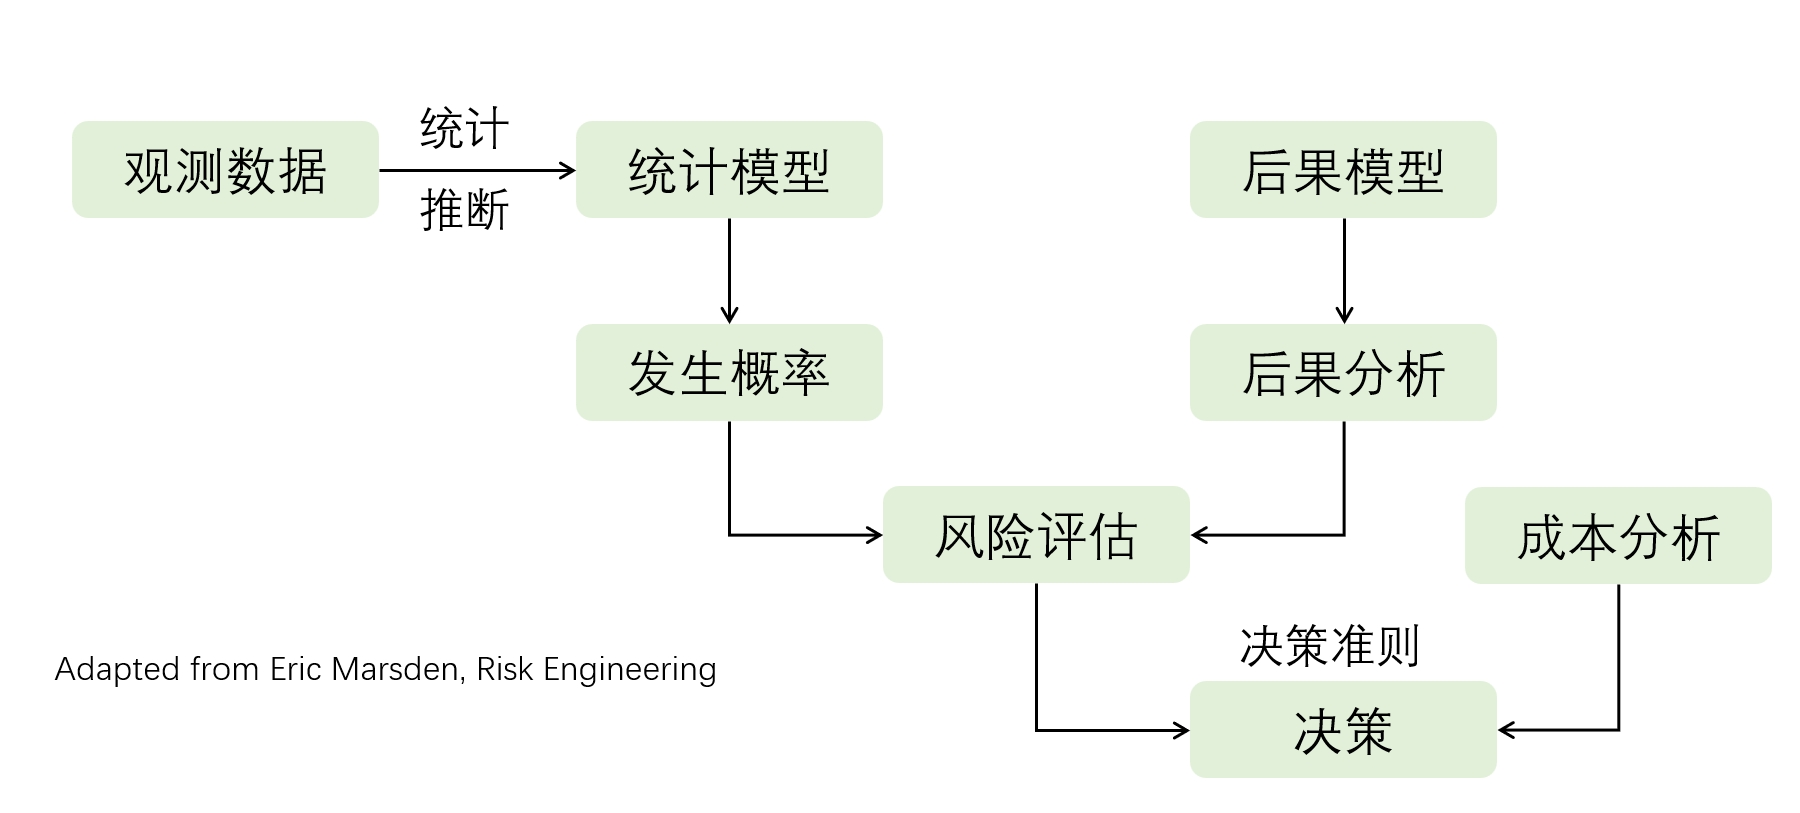
\includegraphics[width=0.8\textwidth]{pic/2.0.1.png}
    \caption{决策过程的主要环节}
\end{figure}


\section{线性回归(Linear Regression)}

\textbf{回归分析}:研究因变量(dependent variable)与自变量(independent variable)之间关联关系。线性回归(Linear Regression)是最基本的回归分析方法。

\textbf{线性回归}:假设因变量$y$与自变量$x_{11},x_{12},\cdots,x_{nn}$之间满足线性关系,即
\begin{equation}
    y = X\beta + \varepsilon
\end{equation}
用矩阵形式表示为
\begin{equation}
    \begin{bmatrix}
        y_1    \\
        y_2 \
        \vdots \\
        y_n
    \end{bmatrix}
    =
    \begin{bmatrix}
        x_{11} & x_{12} & \cdots & x_{1n} \\
        x_{21} & x_{22} & \cdots & x_{2n} \\
        \vdots & \vdots & \ddots & \vdots \\
        x_{n1} & x_{n2} & \cdots & x_{nn}
    \end{bmatrix}
    \begin{bmatrix}
        \beta_1 \\
        \beta_2 \\
        \vdots  \\
        \beta_n
    \end{bmatrix}
    +
    \begin{bmatrix}
        \varepsilon_1 \\
        \varepsilon_2 \\
        \vdots        \\
        \varepsilon_n
    \end{bmatrix}
\end{equation}
其中
\begin{enumerate}[itemsep=0pt,parsep=0pt]
    \item $y$ 为因变量向量,也被称为响应变量(response variable),被解释变量(explained variable)等。
    \item $X$为自变量矩阵,也被称为解释变量(explanatory variable),预测变量“predictor variable”,协变量(covariate variable)等。
    \item $\beta$ 为回归系数向量(vector of regression coefficients)。
    \item $\varepsilon$ 为剩余误差向量(residual errors),也称残差、残余误差等,包含了因变量$\mathbf{y}$无法被自变量$X$解释的部分。
\end{enumerate}

\subsection{普通最小二乘法OLSR}

普通最小二乘法(Ordinary Least Square Regression, OLSR)是线性回归的基本方法。

通常使用普通最小二乘方法估计回归系数$\beta$,该系数最小化剩余误差方差。

\subsection{OLS的假设}

普通最小二乘法主要基于以下假设:

\textbf{1.线性函数形式}:因变量$y$与自变量$X$之间为线性关系。

利用散点图或者相关系数可以初步判断因变量与自变量之间是否存在线性关系。

\textbf{2.剩余误差独立同分布}:利用数据进行模型拟合后,模型的剩余误差应该为独立同分布的随机变量。

剩余误差应该为随机变量,使用不同数据拟合模型后的剩余误差是随机的,因此为随机变量;

残余误差应相互独立,可以通过残余误差与自变量,或者残余误差与因变量之间的散点图进行观测;

不同观测值的残余误差应该服从相同的分布。

\textbf{3.剩余误差呈正态分布}:剩余误差应该呈现正态分布。

普通最小二乘法的统计检验和显著性分析都基于正态分布假设。

\textbf{4.剩余误差同方差(homoscedastic)}:剩余误差应该有近似常数的方差,方差不依赖自变量变化。

\begin{figure}[h]
    \centering
    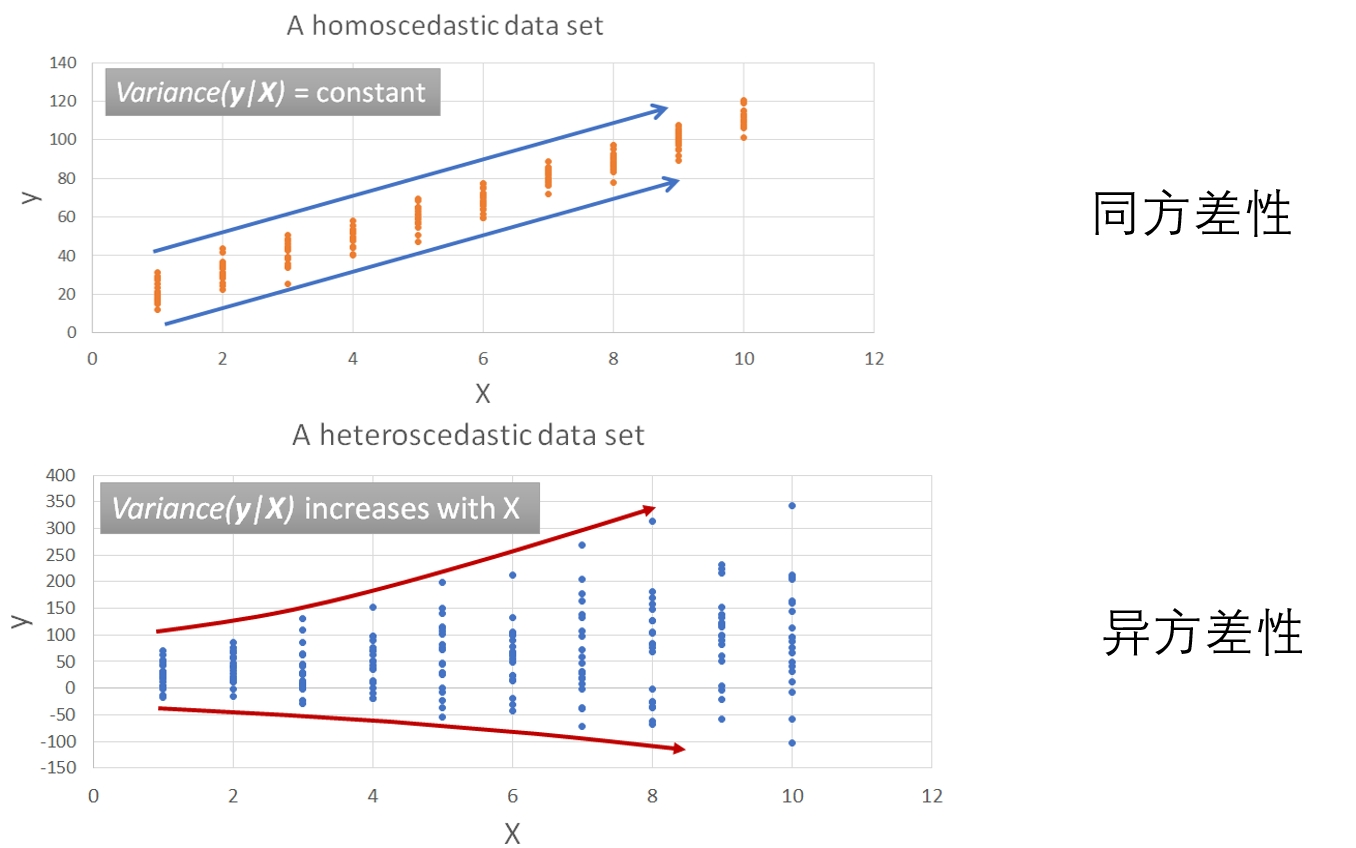
\includegraphics[width=0.8\textwidth]{pic/2.1.1.png}
    \caption{同方差性}
\end{figure}

\subsection{OLS的剩余误差方差}

通常使用普通最小二乘方法估计回归系数$\beta$,该系数最小化剩余误差方差。

剩余误差方差估计为
\begin{equation}
    Var(\varepsilon | X) = \frac{\left(\varepsilon - E(\varepsilon | X)\right)^T\left(\varepsilon - E(\varepsilon | X)\right)}{n-k}
\end{equation}
其中$n$为样本量,$k$为自由变量个数。从前面普通最小二乘法假设可知,剩余误差呈均值为0的正态分布,并且与任何自变量无关,因此有$E(\varepsilon | X) = 0$,剩余误差方差估计为
\begin{equation}
    Var(\varepsilon | X) = \frac{\varepsilon^T\varepsilon}{n-k}
\end{equation}

如果我们计算出最佳回归系数$\hat{\beta}$,则可以计算出预测值$\hat{y}$,预测值与真实值之间的误差为
\begin{equation}
    \begin{aligned}
        e & = y - \hat{y}      \\
          & = y - X\hat{\beta}
    \end{aligned}
\end{equation}
从而
\begin{equation}
    \begin{aligned}
        Var(\varepsilon | X) & = \frac{e^Te}{n-k}                                   \\
                             & = \frac{(y - X\hat{\beta})^T(y - X\hat{\beta})}{n-k}
    \end{aligned}
\end{equation}

最小化剩余误差方差,等效于最小化$e^Te$,即
\begin{equation}
    \hat{\beta} = \arg \min_{\beta} e^Te = \arg \min_{\beta} (y - X\beta)^T(y - X\beta)
\end{equation}

对目标方程求导,令其等于0,进行求解
\begin{equation}
    \begin{aligned}
        \frac{\partial e^Te}{\partial \beta} & = \frac{\partial (y - X\beta)^T(y - X\beta)}{\partial \beta} \\
                                             & = -2X^T(y - X\beta) = 0
    \end{aligned}
\end{equation}
从而
\begin{equation}
    \hat{\beta} = (X^TX)^{-1}X^Ty
\end{equation}
这就是线性回归的普通最小二乘估计。

\subsection{OLS的协方差矩阵(covariance matrix)}

注意到
\begin{equation}
    \hat{\beta} = (X^TX)^{-1}X^Ty = (X^TX)^{-1}X^T(X\beta + \varepsilon) = \beta + (X^TX)^{-1}X^T\varepsilon
\end{equation}

OLS的协方差矩阵为
\begin{equation}
    \begin{aligned}
        Var(\hat{\beta}) & = Var((X^TX)^{-1}X^Ty)                                  \\
                         & = E((X^TX)^{-1}X^T\varepsilon\varepsilon^TX(X^TX)^{-1}) \\
                         & = (X^TX)^{-1}X^TVar(\varepsilon)X(X^TX)^{-1}            \\
                         & = (X^TX)^{-1}X^T\sigma^2IX(X^TX)^{-1}                   \\
                         & = \sigma^2 (X^TX)^{-1}
    \end{aligned}
\end{equation}
其中用到了剩余误差独立同分布、同方差(homoscedastic)假设:$Var(\varepsilon) = \sigma^2I$。

$e$是对剩余误差$\varepsilon$的无偏估计可以根据拟合结果的残差估计$\sigma$
\begin{equation}
    \sigma^2 = s^2  = \frac{e^Te}{n-k} = \frac{(y - X\hat{\beta})^T(y - X\hat{\beta})}{n-k}
\end{equation}

\begin{note}
    如果数据和拟合结果不满足上面的条件,会发生什么呢?

    拟合结果不能很好地描述我们的数据特征,比如如果数据的方差随均值变化,那么我们使用普通最小二乘法,剩余误差很难满足独立同分布和同方差假设,我们选用的方法就是不最优的方法。

    在推导置信区间时,我们使用了以上假设,无法使用以上关系获得置信区间。
\end{note}

\section{离散数据}

离散数据通常称为分类数据,因为可以将观测值收集到不同的类别中。离散变量一般可以分为以下几种类型:

\begin{enumerate}[itemsep=0pt,parsep=0pt]
    \item 定类 (Nominal variable):变量的不同取值仅仅代表处于不同类别,例如性别、国籍、职业等,数值一般没有实际意义。
    \item 定序 (Ordinal variable) :变量的值不仅能够代表类别,还能代表某种特性的排序,例如满意程度、教育程度等,定序变量的值之间可以比较大小,但数值之差一般没有实际意义。
    \item 定量(Quantitative variable):变量的值代表可数的数量,例如单位时间内交通事故、火灾事故数量、年龄、收入等,定量变量的数值具有实际意义,差值或者比值也具有实际意义。

          定量数据可以进一步依据数据是否可以相减或者相除,可进一步分为定距变量(Interval variable)和定比变量( Ratio variable),但一般不加以区分。
\end{enumerate}

定类和定序变量,其自身数值是没有实际意义的,但是如果统计每一类别的频次(Frequency Counts),则数值具有实际意义;

频次的统计一般可以表示为两个或者多个变量的联合形式(jointly)或者边际形式(marginally)。

\begin{note}
    统计眼睛颜色:眼睛颜色可以认为是定类变量(Nominal variable);可以统计每一类别的频次。

    入学申请结果:灰色区域为两个变量的联合形式数据;黄色区域为边际形式数据。

    \begin{table}[h]
        \centering
        \setlength{\tabcolsep}{5mm}
        \begin{tabular}{ccc|c}
            \hline
                                    & \cellcolor{gray!25}男     & \cellcolor{gray!25}女     & \cellcolor{yellow!25} 总计 \\
            \hline
            \cellcolor{gray!25}通过   & \cellcolor{gray!25}100   & \cellcolor{gray!25}50    & \cellcolor{yellow!25}150 \\
            \cellcolor{gray!25}拒绝   & \cellcolor{gray!25}50    & \cellcolor{gray!25}100   & \cellcolor{yellow!25}150 \\
            \hline
            \cellcolor{yellow!25}总计 & \cellcolor{yellow!25}150 & \cellcolor{yellow!25}150 & \cellcolor{yellow!25}300 \\
            \hline
        \end{tabular}
        \caption{入学申请结果}
    \end{table}


\end{note}

\section{离散数据建模}

\subsection{离散概率分布}

对数据进行统计推断(Statistical inference)或者统计建模时,需要对产生数据的概率分布进行假设,因此,需要首先了解常用的离散数据概率分布。

离散随机变量$X$的概率分布一般使用概率质量函数(PMF,Probability Mass Function)描述
\begin{equation}
    P(X = x) = f(x)
\end{equation}

使得$f(x)>0$的$x$的集合被称为函数的支集(Support set),概率质量函数在这个集合上不为零,这个集合“支撑”了这个函数的非零值。

如果概率分布依赖某个未知参数$\theta$,可以将概率质量函数记为
\begin{equation}
    P(X = x | \theta) = f(x | \theta)
\end{equation}

\subsubsection{概率质量函数(PMF)}

概率质量函数(PMF)描述的是离散随机变量在各个特定取值上的概率,比如一颗均匀的骰子,1到6出现的概率是1/6,概率质量函数为
\begin{equation}
    f(x) = \frac{1}{6}, x = 1,2,3,4,5,6
\end{equation}

再比如抛硬币,正面得1分,反面得0分,抛2次硬币,得分就是随机变量,它的概率质量函数为
\begin{equation}
    f(x) = \begin{cases}
        \frac{1}{4}, & x = 0,2   \\
        \frac{1}{2}, & x = 1     \\
        0,           & \text{其他}
    \end{cases}
\end{equation}

\subsubsection{概率密度函数(PDF)}

概率密度函数(PDF)是描述连续随机变量的分布,它本身不是概率,只有对连续随机变量的取值进行积分后才得到概率。

例如,正态分布的概率密度函数为
\begin{equation}
    f(x) = \frac{1}{\sqrt{2\pi}\sigma}e^{-\frac{(x-\mu)^2}{2\sigma^2}}
\end{equation}

\subsection{常用离散概率分布}

\begin{itemize}[itemsep=0pt,parsep=0pt]
    \item 伯努利分布(Bernoulli distribution)
    \item 二项分布(Binomial distribution)
    \item 泊松分布(Poisson distribution)
    \item 负二项分布(Negative-Binomial distribution)
    \item 超几何分布(Hypergeometric distribution)
    \item 多项式分布(Multinomial distribution)
\end{itemize}

\subsubsection{伯努利分布(Bernoulli Distribution)}

伯努利分布是最基本的离散随机变量概率分布。

\textbf{伯努利试验(Bernoulli experiment)}

\begin{itemize}[itemsep=0pt,parsep=0pt]
    \item 在同样的条件下重复地、相互独立地进行的一系列随机试验;
    \item 每次试验假设该项试验独立重复地进行了n次,那么就称这一系列重复独立的随机试验为$n$重伯努利试验。
\end{itemize}

伯努利试验是单次随机试验,只有两种结果,例如0或1,成功或失败,黑或白,正或反。其概率分布称为伯努利分布(Bernoulli distribution),也成为0-1分布,是最简单的离散概率分布。

\textbf{伯努利分布(Bernoulli distribution)}

离散随机变量$X$可取$0$和$1$两个值,如果$X=1$出现的概率为$\pi$, $X=0$出现的概率为$1-\pi$,则称该变量服从伯努利分布
\begin{equation}
    P(X = x) = \pi^x(1-\pi)^{1-x}, x = 0,1
\end{equation}

期望(mean or expected value)为
\begin{equation}
    E(X) = 1 \cdot \pi + 0 \cdot (1-\pi) = \pi
\end{equation}

方差(variance)为
\begin{equation}
    Var(X) = E(X^2) - E(X)^2 = \pi - \pi^2 = \pi(1-\pi)
\end{equation}

\subsubsection{二项分布(Binomial Distribution)}

$X_1,X_2,...,X_n$为独立同分布的伯努利随机变量,都服从
\begin{equation}
    P(X_i = 1) = \pi, P(X_i = 0) = 1 - \pi
\end{equation}
令$X = X_1 + X_2 + \cdots + X_n$,则$X$服从二项分布(Binomial distribution),记为
\begin{equation}
    X \sim Bin(n, \pi)
\end{equation}

\begin{example}
    将一枚均质的硬币抛100次,观察到正面次数为随机变量$X$,$X$服从二项分布$X \sim Bin(100, 0.5)$
\end{example}

二项分布的概率质量函数(PMF)为
\begin{equation}
    P(X = x) = \binom{n}{x}\pi^x(1-\pi)^{n-x}, x = 0,1,2,\cdots,n
\end{equation}

期望为
\begin{equation}
    E(X) = \sum_{x=0}^n x \binom{n}{x}\pi^x(1-\pi)^{n-x} = \sum_{i=1}^n E(X_i) = n\pi
\end{equation}

方差为
\begin{equation}
    \begin{aligned}
        Var(X) & = \sum_{x=0}^n (x - E(X))^2 \binom{n}{x}\pi^x(1-\pi)^{n-x} \\
               & = \sum_{i=1}^n Var(X_i) = n\pi(1-\pi)
    \end{aligned}
\end{equation}

\subsubsection{泊松分布(Poisson Distribution)}

泊松分布是二项分布的一种特殊情况,当$n$很大,$\pi$很小时,二项分布可以近似为泊松分布。

\begin{example}
    泊松分布适合于描述单位时间内随机事件发生的次数的概率分布。如某一服务设施在一定时间内受到的服务请求的次数,电话交换机接到呼叫的次数、汽车站台的候客人数、机器出现的故障数、自然灾害发生的次数、DNA序列的变异数、放射性原子核的衰变数、激光的光子数分布等等。(单位时间内发生的次数,可以看作事件发生的频率,类似物理的频率$f$)。
\end{example}

长期来看,每固定时间段内发生事故平均次数(或事故发生率)基本恒定为$\lambda$,同时事件之间相互独立,则称$X$服从参数为$\lambda$的泊松分布,记为
\begin{equation}
    X \sim Poisson(\lambda)
\end{equation}

泊松分布的概率质量函数(PMF)为
\begin{equation}
    P(X = x) = \frac{\lambda^x}{x!}e^{-\lambda}, x = 0,1,2,\cdots
\end{equation}

泊松分布事实上是二项分布的极限情况,当$n$很大,$\pi$很小时,二项分布可以近似为泊松分布:
\begin{equation}
    \begin{aligned}
        P(X = x) & = \lim_{n \to \infty} \binom{n}{x}\pi^x(1-\pi)^{n-x}                                                                                         \\
                 & = \lim_{n \to \infty} \frac{n(n-1)\cdots(n-x+1)}{x!}\pi^x(1-\pi)^{n-x}                                                                       \\
                 & = \lim_{n \to \infty} \frac{n^x}{x!}\left(1-\frac{1}{n}\right)\left(1-\frac{2}{n}\right)\cdots\left(1-\frac{x-1}{n}\right)\pi^x(1-\pi)^{n-x} \\
                 & = \lim_{n \to \infty} \frac{n^x}{x!}\pi^x\left(1-\frac{\lambda}{n}\right)^n\left(1-\frac{\lambda}{n}\right)^{-x}                             \\
                 & = \frac{\lambda^x}{x!}e^{-\lambda}
    \end{aligned}
\end{equation}
其中$\lambda = n\pi$。

\begin{note}
    泊松分布也有相应的前提假设:
    \begin{enumerate}[itemsep=0pt,parsep=0pt]
        \item 事件发生的概率很小,即$\pi$很小;
        \item 事件发生的次数很大,即$n$很大。
    \end{enumerate}


    如前所述,泊松分布要求事件发生率保持恒定,比如发生交通事故的频率;(但需要注意的是,我们在对数据进行建模的时候,可以根据相关变量对事件发生率进行估计和调整,即不同环境或者变量对应的发生率可以变化);

    事件需要相互独立,例如前面交通事故的发生不会对后面的交通事故是否发生造成影响。
\end{note}

期望为
\begin{equation}
    E(X) = \sum_{x=0}^{\infty} x \frac{\lambda^x}{x!}e^{-\lambda} = \lambda
\end{equation}

方差为
\begin{equation}
    \begin{aligned}
        Var(X) & = \sum_{x=0}^{\infty} (x - E(X))^2 \frac{\lambda^x}{x!}e^{-\lambda} \\
               & = \lambda
    \end{aligned}
\end{equation}
可以看到,泊松分布的期望和方差相等。

\begin{note}
    在对数据进行统计建模时,这一限制通常过于严格,方差大于均值时为过分散(overdispersion),方差小于均值时称为欠分散(underdispersion),对于这类数据则需要对泊松假设进行调整,或者采用其他离散分布,一般负二项分布是比较好的备选。
\end{note}

泊松分布是一种描述和分析稀有事件的概率分布,要观察这类事件$n$要足够大。

泊松分布所依赖的唯一参数$\lambda$,其值越小,分布越偏倚,随着$\lambda$的增大,分布越对称,当$\lambda \geqslant 50$时可用正态分布近似处理泊松分布问题。

如下图所示,当$\lambda$较小时,泊松分布呈现偏倚态,当$\lambda$较大时,泊松分布呈现对称态。

\begin{figure}[h]
    \centering
    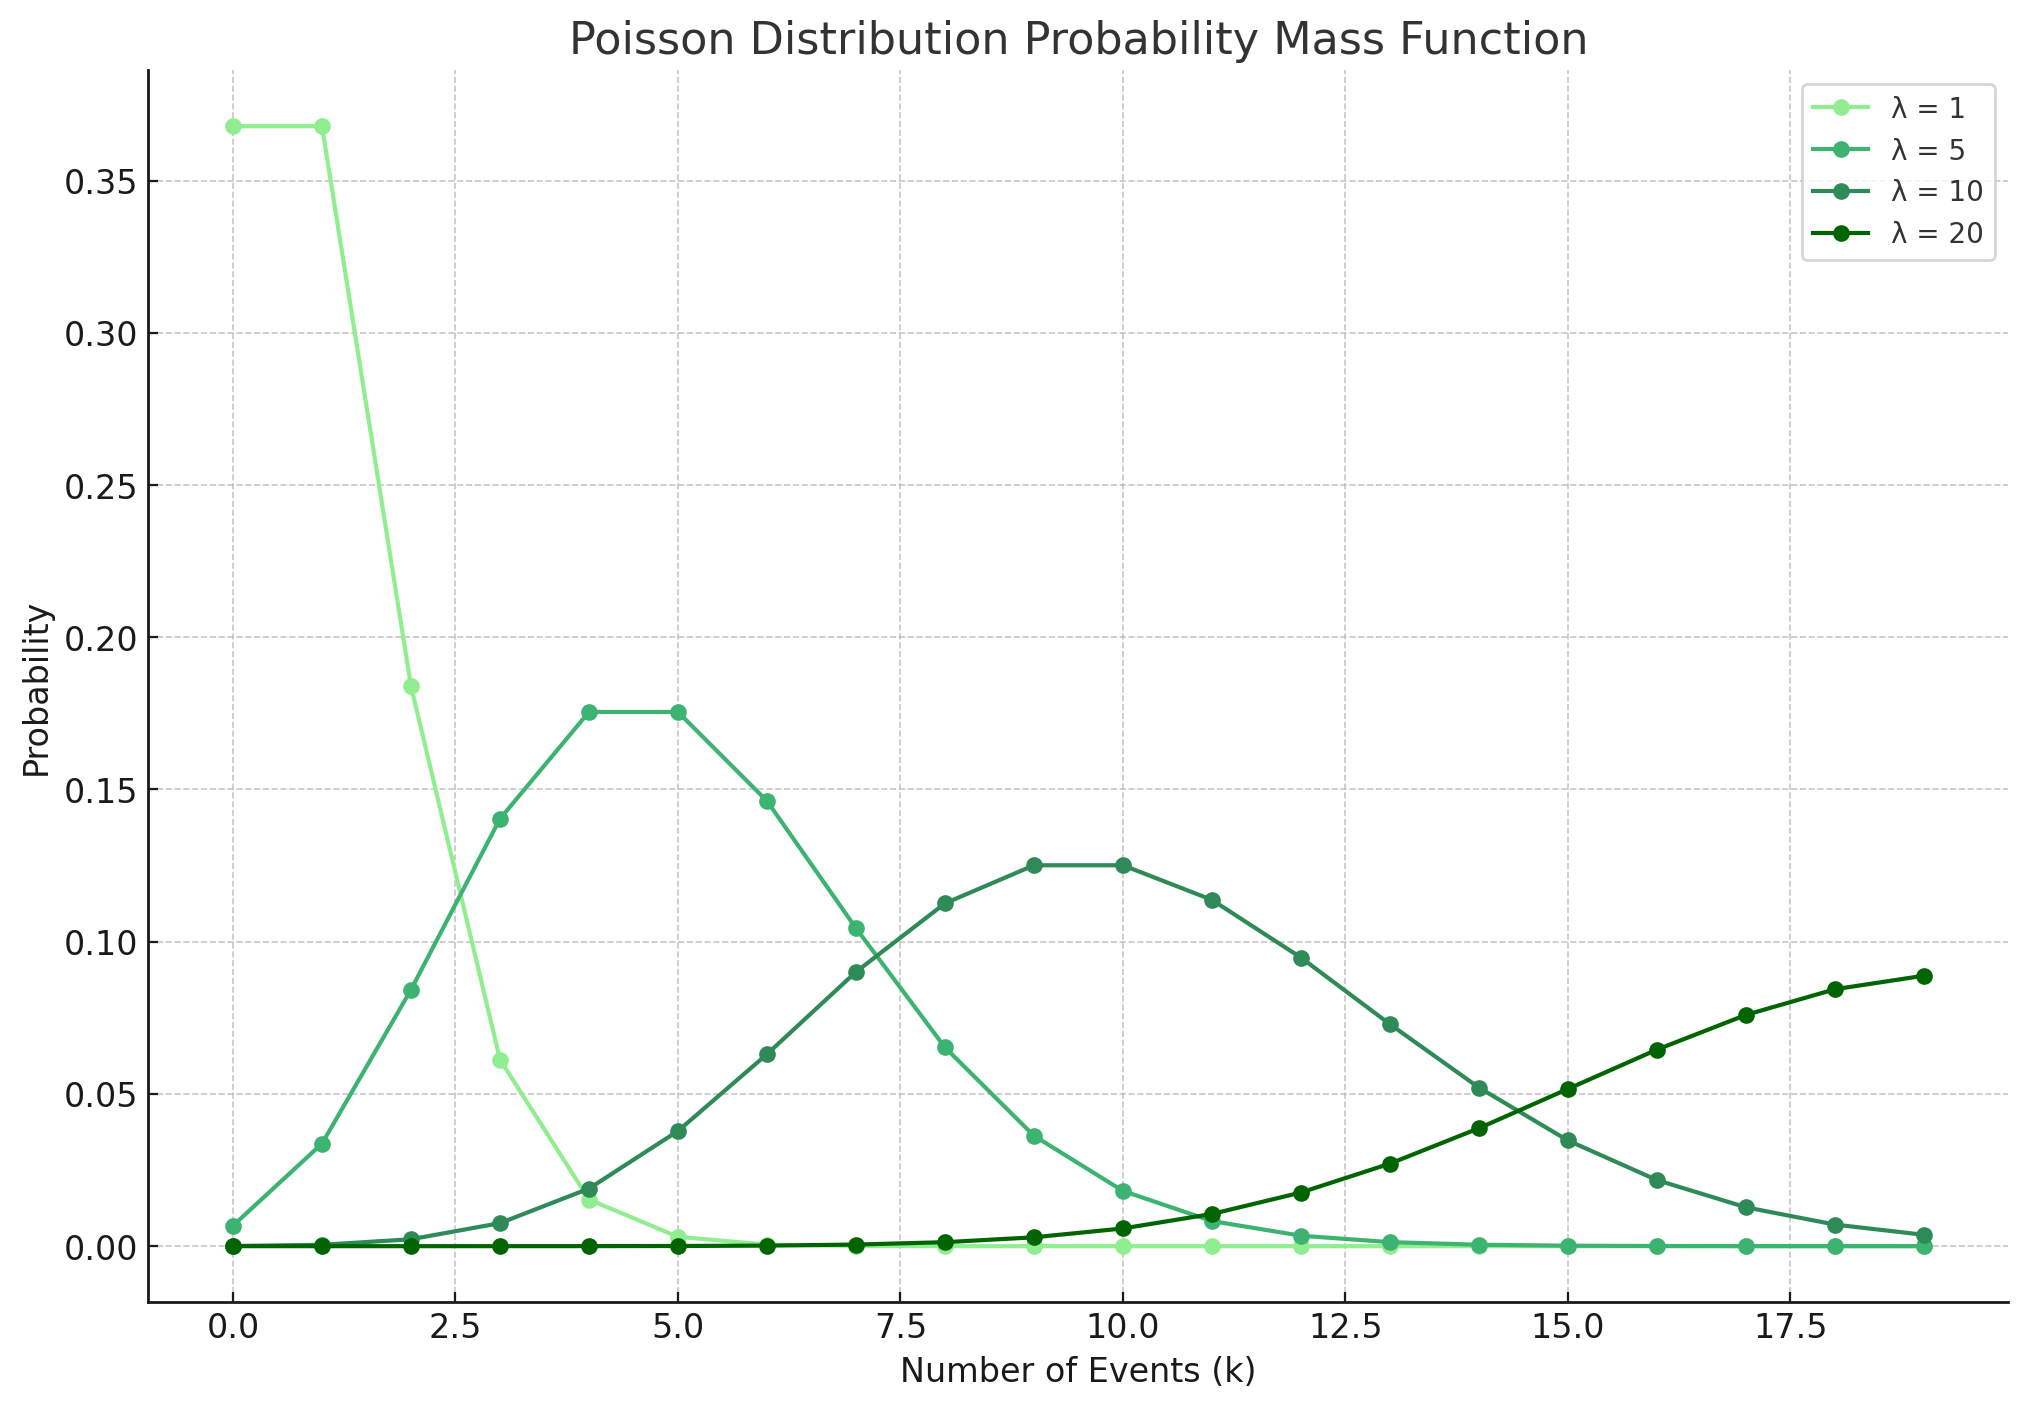
\includegraphics[width=0.8\textwidth]{pic/2.3.1.png}
    \caption{泊松分布}
\end{figure}

\subsubsection{负二项分布(Negative-Binomial Distribution)}

负二项分布是二项分布的推广,二项分布是$n$重伯努利试验中成功次数的分布,负二项分布是$n$重伯努利试验中成功次数$X$的分布。

负二项分布与二项分布类似,但其描述的是在出现固定“失败”次数$r$之前,成功的次数$x$。

\begin{example}
    同样是抛硬币,负二项分布描述的是在出现100次背面之前,正面出现次数的分布。
\end{example}

负二项分布的概率质量函数PMF为
\begin{equation}
    P(X = x) = \binom{x+r-1}{x}\pi^r(1-\pi)^x, x = 0,1,2,\cdots
\end{equation}

与泊松分布类似,负二项分布同样是对一段时间或某一区域内,事件发生频次统计建模的重要离散分布。但负二项分布包含两个参数,$r$和$π$,其期望和方差分别为:
\begin{equation}
    E(X) = \frac{r(1-\pi)}{\pi} = \mu
\end{equation}
\begin{equation}
    Var(X) = \frac{r(1-\pi)}{\pi^2} = \mu + \frac{\mu^2}{r}
\end{equation}

负二项分布不再要求均值和方差相同,相对较弱的限制条件,也使得负二项分布可以对数据进行较好的拟合。

\subsubsection{超几何分布(Hypergeometric Distribution)}

假设总体包含$n$个个体,每个个体具有两种类型,类型1和类型2:类型1的个数为$n_1$,类型2的个数为$n_2=n-n_1$。

从总体中抽取$m$个样本,则其中类型1的个数$X$为随机变量,并服从超几何分布,其概率质量函数PMF为
\begin{equation}
    P(X = x) = \frac{\binom{n_1}{x}\binom{n_2}{m-x}}{\binom{n}{m}}, x \in [max(0, m-n_2), min(m, n_1)]
\end{equation}

超几何分布的期望和方差分别为
\begin{equation}
    E(X) = \frac{mn_1}{n}
\end{equation}
\begin{equation}
    Var(X) = \frac{mn_1n_2(n-m)}{n^2(n-1)}
\end{equation}

\subsubsection{多项式分布(Multinomial Distribution)}

多项分布是对二项分布的拓展,包含$k$类不同的结果,每类结果出现的概率分别为$\pi_1,\pi_2,\cdots,\pi_k$,则多项式分布的概率质量函数PMF为
\begin{equation}
    P(X_1 = x_1, X_2 = x_2, \cdots, X_k = x_k) = \frac{n!}{x_1!x_2!\cdots x_k!}\pi_1^{x_1}\pi_2^{x_2}\cdots\pi_k^{x_k}
\end{equation}
其中$x_1,x_2,\cdots,x_k$满足
\begin{equation}
    \sum_{i=1}^k x_i = n
\end{equation}

多项式分布的期望和方差分别为
\begin{equation}
    E(X_i) = n\pi_i
\end{equation}
\begin{equation}
    Var(X_i) = n\pi_i(1-\pi_i)
\end{equation}

\section{最大似然估计(Maximum Likelihood Estimation, MLE)}

\subsection{似然函数(Likelihood function)}

似然(Likelihood)或似然函数(Likelihood function)是现代统计最为基础的概念之一。

在前面介绍的离散随机变量分布中,通常具有一个或者多个参数,例如泊松分布中的事件发生率$\lambda$、二项分布中的事件概率$\pi$(二项分布中的$n$一般是固定的)。

在针对实际问题的统计分析中,我们通常假设已经获取的数据服从某种分布,因此分布中的参数通常是未知的,需要通过数据来估计未知参数。

似然函数(Likelihood function)是观测数据的联合概率与所选取的统计模型所包含的参数之间的函数,表示模型参数的似然性(Likelihood)。

似然函数可以理解为一种条件概率:假设事件$A$发生(可以是多个事件的联合概率),估计参数$B$(可以是多个参数组成的向量)选取不同值的可能性,可以表示为似然函数
\begin{equation}
    L(B|A) = P(A|B)
\end{equation}

对于某一参数$b$对应的似然性,可以采用条件概率函数估计
\begin{equation}
    L(b|A) = P(A|B=b)
\end{equation}

需要指出的是,并不要求似然函数满足归一性,一个似然函数乘以正的常数,依然是似然函数
\begin{equation}
    L(b|A) = cP(A|B=b) , c > 0
\end{equation}

\begin{note}
    似然性(Likelihood)与概率(Probability)

    似然性(Likelihood)与概率(Probability)在字面上具有相似的含义,都是指某事件发生的可能性,但是统计学中,二者有显著的区别:

    \begin{enumerate}[itemsep=0pt,parsep=0pt]
        \item 概率(Probability):假设观测数据服从某种概率密度分布,在相应的概率模型参数已知的情况下,获得的某一特定观测结果出现的可能性,即统计模型和参数已知,估计观测出现的可能性。
        \item 似然性(Likelihood):同样假设观测数据服从某种概率密度分布,相应的概率模型参数未知,但具有观测数据,即具有服从该分布的采样数据,衡量某种统计模型参数导致所获得的观测数据出现的可能性,即统计模型和观测数据已知,估计模型参数导致观测结果的可能性。
    \end{enumerate}

    似然性(Likelihood)与概率(Probability)的区别可以通过下面的例子进行理解,以掷硬币伯努利试验为例:

    \begin{enumerate}[itemsep=0pt,parsep=0pt]
        \item 概率(Probability):假设硬币完全均质($\pi =0.5$),抛一次硬币出现正面的概率为$0.5$
        \item 似然性(Likelihood):首先进行观测试验,抛$100$次硬币,其中仅出现了$10$次正面,此时可以认为,

              假设硬币均质($\pi =0.5$)的似然性较低($P=1.37\times 10^{-17}$);
              假设硬币均质($\pi =0.1$)的似然性较高($P=0.13$)。


    \end{enumerate}

    从上面的例子可以看出,概率(Probability)是对于已知的参数,估计观测结果的可能性;似然性(Likelihood)是对于已知的观测结果,估计参数的可能性。
\end{note}

\subsubsection{伯努利分布的似然函数}

假设进行$n$次伯努利试验,则有$n$个伯努利随机变量$X_1,X_2,\cdots,X_n$,每个随机变量都有概率质量
\begin{equation}
    P(X_i = x_i) = \pi^{x_i}(1-\pi)^{1-x_i}, x_i = 0,1
\end{equation}

此时,似然函数为$n$次试验结果的联合概率密度分布,由于试验相互独立,因此似然函数可表示为:
\begin{equation}
    \begin{aligned}
        L(\pi) & = P(X_1 = x_1, X_2 = x_2, \cdots, X_n = x_n | \pi)                 \\
               & = \prod_{i=1}^n P(X_i = x_i)                                       \\
               & = \prod_{i=1}^n \pi^{x_i}(1-\pi)^{1-x_i}                           \\
               & = \pi^{\sum\limits_{i=1}^n x_i}(1-\pi)^{n-\sum\limits_{i=1}^n x_i}
    \end{aligned}
\end{equation}
注意似然函数是概率模型参数$\pi$的函数,而不是随机变量$X$的函数。

\subsection{最大似然估计(Maximum Likelihood Estimation, MLE)}

概率模型参数有取不同值的可能,但如果存在一个取值,使得概率似然函数达到最大,那么该值就成为该参数在现有观测下的“最合理”参数值。

最大似然估计(Maximum Likelihood Estimation)将能够使似然函数最大化的未知参数的值最为对该参数的估计。

\subsubsection{伯努利分布参数$\pi$的最大似然估计}

伯努利分布的似然函数为
\begin{equation}
    L(\pi) = \pi^{\sum_{i=1}^n x_i}(1-\pi)^{n-\sum_{i=1}^n x_i}
\end{equation}

对似然函数取对数,可以简化计算
\begin{equation}
    \begin{aligned}
        \ln L(\pi) & = \ln \left(\pi^{\sum_{i=1}^n x_i}(1-\pi)^{n-\sum_{i=1}^n x_i}\right) \\
                   & = \sum_{i=1}^n x_i \ln \pi + (n-\sum_{i=1}^n x_i)\ln(1-\pi)
    \end{aligned}
\end{equation}

对似然函数求导,令导数等于0,可以求得最大似然估计
\begin{equation}
    \begin{aligned}
        \frac{\partial \ln L(\pi)}{\partial \pi} & = \frac{\sum\limits_{i=1}^n x_i}{\pi} - \frac{n-\sum_{i=1}^n x_i}{1-\pi} = 0 \\
        \hat{\pi }                               & = \frac{\sum\limits_{i=1}^n x_i}{n}
    \end{aligned}
\end{equation}

\subsubsection{二项分布参数$\pi$的最大似然估计}

二项分布的似然函数为
\begin{equation}
    L(\pi) = \prod_{i=1}^m \binom{n}{x_i}\pi^{x_i}(1-\pi)^{n-x_i}
\end{equation}

对似然函数取对数,可以简化计算
\begin{equation}
    \begin{aligned}
        \ln L(\pi) & = \ln \left(\prod_{i=1}^m \binom{n}{x_i}\pi^{x_i}(1-\pi)^{n-x_i}\right)                       \\
                   & = \sum_{i=1}^m \ln \binom{n}{x_i} + \sum_{i=1}^m x_i \ln \pi + \sum_{i=1}^m (n-x_i)\ln(1-\pi)
    \end{aligned}
\end{equation}

对似然函数求导,令导数等于0,可以求得最大似然估计
\begin{equation}
    \begin{aligned}
        \frac{\partial \ln L(\pi)}{\partial \pi} & = \frac{\sum\limits_{i=1}^m x_i}{\pi} - \frac{m-\sum_{i=1}^m x_i}{1-\pi} = 0 \\
        \hat{\pi }                               & = \frac{\sum\limits_{i=1}^m x_i}{mn}
    \end{aligned}
\end{equation}

\subsubsection{泊松分布参数$\lambda$的最大似然估计}

泊松分布的似然函数为
\begin{equation}
    L(\lambda) = \prod_{i=1}^n \frac{\lambda^{x_i}}{x_i!}e^{-\lambda}
\end{equation}

对似然函数取对数,可以简化计算
\begin{equation}
    \begin{aligned}
        \ln L(\lambda) & = \ln \left(\prod_{i=1}^n \frac{\lambda^{x_i}}{x_i!}e^{-\lambda}\right)      \\
                       & = \sum_{i=1}^n \ln \frac{\lambda^{x_i}}{x_i!} + \sum\limits_{i=1}^n -\lambda \\
                       & = \sum_{i=1}^n x_i \ln \lambda - \sum\limits_{i=1}^n \ln x_i! - n\lambda
    \end{aligned}
\end{equation}

对似然函数求导,令导数等于0,可以求得最大似然估计
\begin{equation}
    \begin{aligned}
        \frac{\partial \ln L(\lambda)}{\partial \lambda} & = \frac{\sum\limits_{i=1}^n x_i}{\lambda} - n = 0 \\
        \hat{\lambda }                                   & = \frac{\sum\limits_{i=1}^n x_i}{n}
    \end{aligned}
\end{equation}

\subsection{最小二乘法与极大似然估计}

设$y_1,y_2,\cdots,y_n$是来自正态分布$N(\mu,\sigma^2)$的样本,其中$\mu$和$\sigma^2$均未知,求$\mu$和$\sigma^2$的极大似然估计。

正态分布的概率密度函数为
\begin{equation}
    f(x) = \frac{1}{\sqrt{2\pi}\sigma}e^{-\frac{(x-\mu)^2}{2\sigma^2}}
\end{equation}

似然函数为
\begin{equation}
    \begin{aligned}
        L(\mu,\sigma^2) & = \prod_{i=1}^n \frac{1}{\sqrt{2\pi}\sigma}e^{-\frac{
        (y_i-\mu)^2}{2\sigma^2}}                                                  \\
                        & = \left(\frac{1}{\sqrt{2\pi}\sigma}\right)^n e^{-\frac{
                    \sum\limits_{i=1}^n(y_i-\mu)^2}{2\sigma^2}}
    \end{aligned}
\end{equation}

假设方差$\sigma^2$已知,则最大化似然函数等价于最大化指数部分,等价于最小化
\begin{equation}
    \sum_{i=1}^n(y_i-\mu)^2
\end{equation}

\subsection{最大似然方差}

设$n$个样本$x_1,x_2,\cdots,x_n$,独立同分布,均服从具有参数$\theta$的概率分布函数$f_\theta(x)$,样本$x_i$ 时,其对数形式的似然函数可以表示为
\begin{equation}
    L_i(\theta) = \ln f_\theta(x_i)
\end{equation}
$n$个变量的联合概率分布函数为
\begin{equation}
    f_\theta(x_1,x_2,\cdots,x_n) = \prod_{i=1}^n f_\theta(x_i)
\end{equation}
从而对数形式的似然函数
\begin{equation}
    L(\theta) = \ln f_\theta(x_1,x_2,\cdots,x_n) = \sum_{i=1}^n \ln f_\theta(x_i)
\end{equation}


最大似然估计的方差可以通过似然函数的二阶导数来解释
\begin{equation}
    Var(\hat{\theta}) = -\frac{1}{\frac{\partial^2  L(\theta)}{\partial \theta^2}}
\end{equation}

似然函数的二阶导数对应与似然平面(或者曲线)在最大似然估计处的曲率。

\begin{note}
    当曲率较小时,似然平面在最大似然估计附近比较平坦,最大似然估计的方差就比较大,当曲率较大时,似然平面在最大似然估计附近有比较剧烈的弯曲变化,最大似然估计的方差就比较小。
\end{note}

\subsubsection{伯努利分布参数$\pi$的最大似然估计}

伯努利分布的对数似然函数为
\begin{equation}
    L(\pi) = \sum_{i=1}^n x_i \ln \pi + (n-\sum_{i=1}^n x_i)\ln(1-\pi)
\end{equation}

对似然函数求导,令导数等于0,可以求得最大似然估计
\begin{equation}
    \begin{aligned}
        \frac{\partial L(\pi)}{\partial \pi} & = \frac{\sum\limits_{i=1}^n x_i}{\pi} - \frac{n-\sum_{i=1}^n x_i}{1-\pi} = 0 \\
        \hat{\pi }                           & = \frac{\sum\limits_{i=1}^n x_i}{n}
    \end{aligned}
\end{equation}

最大似然估计方差
\begin{equation}
    \begin{aligned}
        Var(\hat{\pi}) & = -\frac{1}{\frac{\partial^2 L(\pi)}{\partial \pi^2}}                                             \\
                       & = -\frac{1}{-\frac{\sum\limits_{i=1}^n x_i}{\pi^2} - \frac{n-\sum\limits_{i=1}^n x_i}{(1-\pi)^2}} \\
                       & = \frac{\pi(1-\pi)}{n}
    \end{aligned}
\end{equation}

\section{广义线性模型(Generalized Linear Models,GLM)}

\subsection{广义线性模型(Generalized Linear Models,GLM)}

广义线性模型(Generalized Linear Models,GLM)是普通最小二乘法的扩展,是用以解决离散因变量、非正态分布因变量的回归分析与建模方法。

广义线性模型假设观测数据因变量$Y$来自某个指数族(exponential family)分布,该分布的均值为$\mu$,均值可以由对应的自变量(解释变量)$X$解释。

因变量Y服从某分布,均值为:
\begin{equation}
    E(Y) = \mu
\end{equation}

均值可被自变量$X$解释,即
\begin{equation}
    \mu = g^{-1}(X\beta)
\end{equation}
其中$g$为连接函数(link function),$\beta$为参数向量。函数$g(.)$通常是非线性的,但解释变量是通过线性组合$X'β$来影响观测值的,基于此种考虑,称其为广义线性模型。

\begin{note}
    指数族(exponential family)分布

    指数族(exponential family)分布是一类常见的概率分布,包括正态分布、泊松分布、二项分布、伽马分布等。

    指数族分布的概率密度函数(PDF)可以表示为
    \begin{equation}
        f(y;\theta,\phi) = \exp \left( \frac{y\theta - b(\theta)}{a(\phi)} + c(y,\phi) \right)
    \end{equation}

    其中:
    \begin{itemize}[itemsep=0pt,parsep=0pt]
        \item \( y \) 是观测值。
        \item \( \theta \) 是自然参数(natural parameter)。
        \item \( \phi \) 是分散参数(dispersion parameter),用于控制分布的变异性。
        \item \( a(\phi) \), \( b(\theta) \) 和 \( c(y,\phi) \) 是特定于分布的函数。
    \end{itemize}

    指数族分布的关键特征在于,它能够用自然参数 \( \theta \) 来表达,而这个参数与观测值的均值 \( \mu \) 之间往往存在一定的关系。在广义线性模型中,我们通常通过链接函数将因变量 \( Y \) 的均值 \( \mu \) 与自变量 \( X \) 关联起来。

    例如:

    \begin{itemize}[itemsep=0pt,parsep=0pt]
        \item 在正态分布中,\( \theta = \mu \),链接函数是恒等函数。
        \item 在二项分布中,\( \theta = \log(\pi/(1-\pi)) \),链接函数是logit函数。
        \item 在泊松分布中,\( \theta = \log(\mu) \),链接函数是自然对数函数。
    \end{itemize}

    通过使用指数族分布,广义线性模型能够适应各种类型的数据,提供灵活而强大的建模框架。

\end{note}

\subsection{GLM的主要成分}

广义线性模型的三个主要成分:

\begin{enumerate}[itemsep=0pt,parsep=0pt]
    \item 随机成分(Random Component),因变量的统计分布,例如普通最小二乘法假设因变量服从正态分布、二值逻辑回归假设因变量服从伯努利分布,随机部分是广义线性模型中唯一的随机性来源。
    \item 系统性成分(Systematic Component),模型的自变量,即解释变量$(x_1,x_2,\cdots,x_n)$,以及他们的线性组合,例如$\beta_0 + \beta_1x_1 + \beta_2x_2 + \cdots + \beta_nx_n$。
    \item 连接函数(Link Function),$\eta$或者$g(\mu)$用以连接广义线性模型的随机成分和系统性成分,表示因变量(响应变量)的均值与自变量(解释变量)之间的关系,例如,在普通最小二乘法中$\eta =g(\mu)=E(Y)$,在逻辑回归中$\eta =g(\pi)=log(\pi/(1- \pi))=logit(\pi)$
\end{enumerate}

\subsection{GLM的假设}

广义线性模型主要假设:
\begin{itemize}[itemsep=0pt,parsep=0pt]
    \item 观测数据因变量$Y_1, Y_2, ..., Y_n$是相互独立的;
    \item 因变量$Y_i$不必服从正态分布,但通常假设其服从某一指数族分布,例如二项分布、泊松分布、负二项分布等;
    \item 因变量与自变量之间不必为线性关系,但一般假设响应变量期望的某种变换(通过连接函数变换)与解释变量之间为线性关系,例如在二值逻辑回归假设$logit(\pi)= \beta_0+ \beta_1x_1+ \beta_2x_2+...+ \beta_nx_n$;可以将原始解释变量的非线性变换作为模型的解释变量;
    \item 响应变量的方差不必是恒定的常数;
    \item 剩余误差需要满足独立条件,但不必为正态分布;
    \item 模型参数利用最大似然估计获得。
\end{itemize}

\subsection{普通最小二乘}

普通最小二乘线性回归可以视为广义线性模型的特例,响应变量$Y$为连续变量
\begin{equation}
    \mu = \beta_0 + \beta_1x_1 + \beta_2x_2 + \cdots + \beta_nx_n
\end{equation}

随机成分:因变量$Y$服从正态分布,正态分布的均值为$\mu$,方差为常数$\sigma^2$;

系统性部分:可以包含多个解释变量,利用解释变量的线性组合来估计响应变量$Y$的期望;

连接函数:线性本体连接(identity), $\eta = g(\mu) = \mu$。

\section{典型的广义线性模型}

\subsection{二值逻辑回归(Logistic Regression)}

二元逻辑回归(Binary Logistic Regression),主要基于解释变量$x_1,x_2,\cdots,x_k$,建立某一事件发生概率($\pi$)的模型。例如
\begin{equation}
    \pi = P(Y=1|X_1=x_1,X_2=x_2,\cdots,X_k=x_k)
\end{equation}

\begin{note}
    根据年龄、血压、收入水平、婚姻状况、吸烟、酗酒情况,估计患有心血管疾病的可能性;

    根据植被覆盖、地表坡度、降雨、土地类型等参数,估计发生滑坡的可能性。
\end{note}

\textbf{二元逻辑回归(Binary Logistic Regression)的主要假设包括}:

因变量(响应变量)$Y$为服从伯努利分布的随机变量,具有“成功”和“失败”两种结果,$Y=1$对应“成功”,出现的概率为$\pi$,$Y=0$对应“失败”,出现的概率为$1-\pi$;

自变量(解释变量)$X= (\mathbf{x}_1,\mathbf{x}_2,\cdots,\mathbf{x}_k)$是固定变量(fixed),可以包含离散变量或者连续变量;

每一个观测样本,例如样本$i$,包含因变量和自变量的值$(x_{1i},x_{2i},\cdots,x_{ki} ,y_i),i=1,\cdots, n$,样本数为$n$个;

不同样本之间相互独立。

\subsubsection{用发生比(odds)估计概率}

\textbf{发生比(odds)},指事件发生的次数/未发生的次数=事件发生的概率/未发生的概率
\begin{equation}
    odds = \frac{\pi}{1-\pi}
\end{equation}
从而
\begin{equation}
    \pi = \frac{odds}{1+odds}
\end{equation}

\textbf{对数发生比,log(odds)},指取$e$为底,真数为odds的自然对数。

\subsubsection{logit函数}

\textbf{二元逻辑回归模型}可以表示为
\begin{equation}
    \ln \left(\frac{\pi_i}{1-\pi_i}\right) = \beta_0 + \bm{\beta}^T \mathbf{x}_i
\end{equation}
其中$\beta_0$为截距,$\beta$为自变量$\mathbf{x}_i$的系数向量。下标$i$对应第$i$个观测值,通过整理可得事件出现概率为
\begin{equation}
    \pi_i = \frac{e^{\beta_0 + \bm{\beta}^T \mathbf{x}_i}}{1+e^{\beta_0 + \bm{\beta}^T \mathbf{x}_i}}
\end{equation}
$n$个$y_1,\cdots,y_n\in \{0,1\}$观测的联合概率,即对数似然函数为
\begin{equation}
    L(\beta_0,\bm{\beta}) = \ln \left(\prod_{i=1}^n \pi_i^{y_i}(1-\pi_i)^{1-y_i}\right)
\end{equation}
通过最大化似然函数,获得最大似然估计$\hat{\beta}_0,\hat{\bm{\beta}}$。

该模型:
\begin{itemize}[itemsep=0pt,parsep=0pt]
    \item 随机成分:因变量(响应变量)Y为服从伯努利分布的随机变量,成功概率为$\pi$,期望$E(Y)= \pi$
    \item 系统性成分:可以包含多个解释变量,利用解释变量的线性组合来估计响应变量$Y$的期望
    \item 连接函数:使用logit函数,$\eta = g(\pi) = \ln \left(\frac{\pi}{1-\pi}\right)$
\end{itemize}

\begin{example}
    \href{https://rpubs.com/beane/n4_1}{研究学习投入时间对考试通过机会的影响}

    收集$6$位同学的投入时间和考试结果如下图

    \begin{figure}[ht]
        \centering
        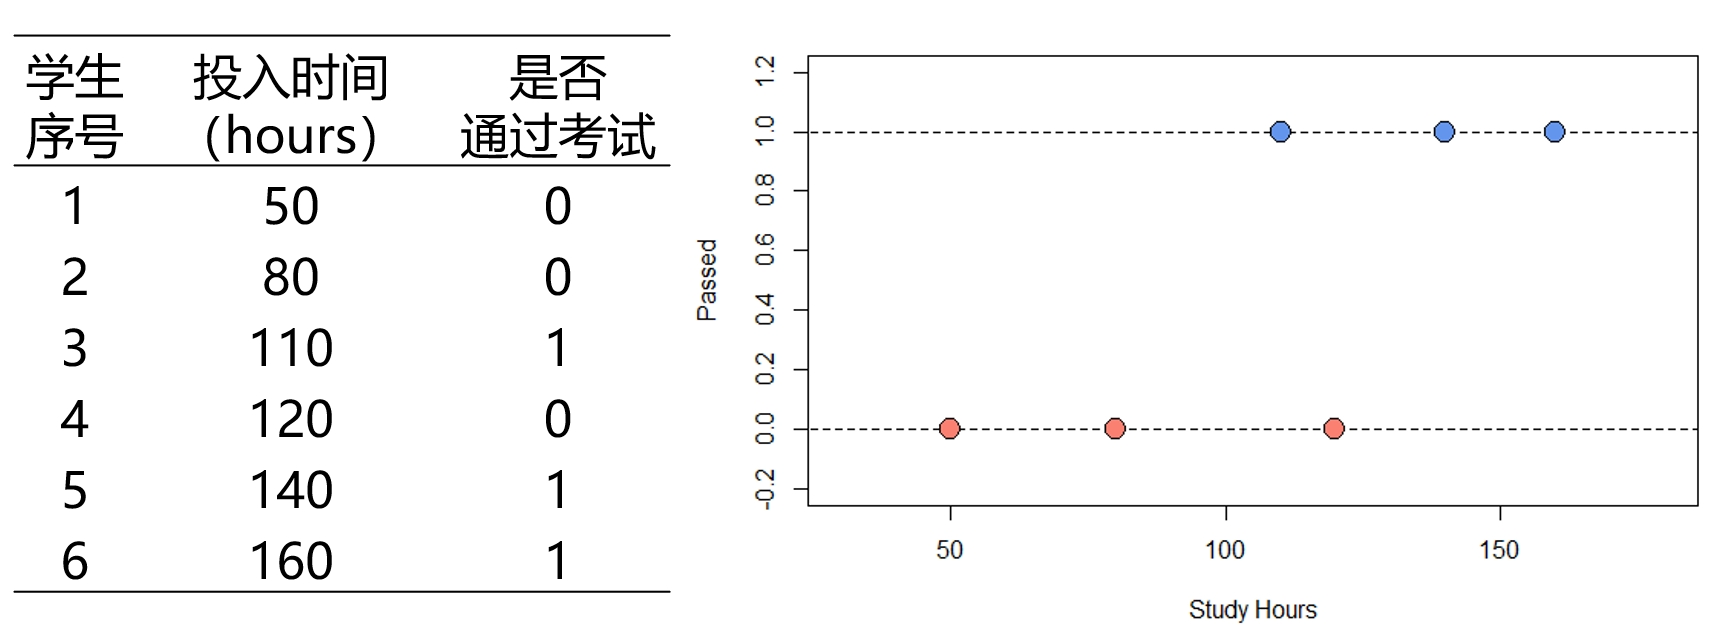
\includegraphics[width=0.8\textwidth]{pic/2.6.1.png}
        \caption{学习投入时间与考试通过机会}
    \end{figure}

    通过二元逻辑回归建立模型,估计学习投入时间对考试通过机会的影响
    \begin{equation}
        \ln \left(\frac{\pi_i}{1-\pi_i}\right) = \beta_0 + \beta_1 x_i
    \end{equation}
    似然函数为
    \begin{equation}
        L(\beta_0,\beta_1) = \ln \left(\prod_{i=1}^n \pi_i^{y_i}(1-\pi_i)^{1-y_i}\right)
    \end{equation}
    通过最大化似然函数,获得最大似然估计$\hat{\beta}_0 = -0.3,\hat{\beta}_1 = 0.082$。

\end{example}

\subsection{泊松回归(Poisson Regression)}

\subsubsection{计数数据}

主要针对\textbf{计数数据(count based data)}进行拟合;

计数数据(count based data):计数数据记录具有一定发生率事件,在一段时间内的出现次数。需要注意的是,事件的发生率可能会随时间或者外界条件的变化而不同
\begin{example}
    一小时内,通过交叉路口的车辆数量;一月内,到医院就诊人数;一年内,北京地区交通事故数量。
\end{example}

计数数据的主要特征:

\begin{itemize}[itemsep=0pt,parsep=0pt]
    \item 离散数据集:数据包含非负整数$[0,+\infty)$,一般回归方法(例如普通最小二乘法等)主要针对实数数据,对离散整数数据的回归分析并非完全合适;
    \item 偏态分布(Skewed distribution):可能在某几个类别中存在大量数据,导致数据出现明显的偏态分布;
    \item 稀疏性(Sparsity):事件出现的频次比较低,比如事故灾害数据,因此数据稀少,呈现稀疏性
    \item 发生率(Rate of occurrence):在对数据建模时,通常假设存在某一发生率$λ$导致观测数据的产生,该发生率可能随时间或者条件的变化而改变。
\end{itemize}

\subsubsection{泊松分布}

泊松分布是对一段时间或某一区域内,事件发生频次统计建模的重要离散分布;通常首先使用泊松回归模型对计数数据进行建模,并将其作为基准模型与其他复杂模型进行对比。

泊松分布的概率质量函数PMF为
\begin{equation}
    P(X=x) = \frac{e^{-\lambda}\lambda^x}{x!}, x=0,1,2,\cdots
\end{equation}
其中随机变量$x$为事件出现的次数,$\lambda$为事件发生率。

泊松分布的一个特点是期望与方差相等,均为$\lambda$,即
\begin{equation}
    E(X) = Var(X) = \lambda
\end{equation}

\subsubsection{泊松回归}

如果事件发生率$\lambda$为常数,那么可以直接使用均值$\lambda$进行预测,如下图所示
\begin{figure}[ht]
    \centering
    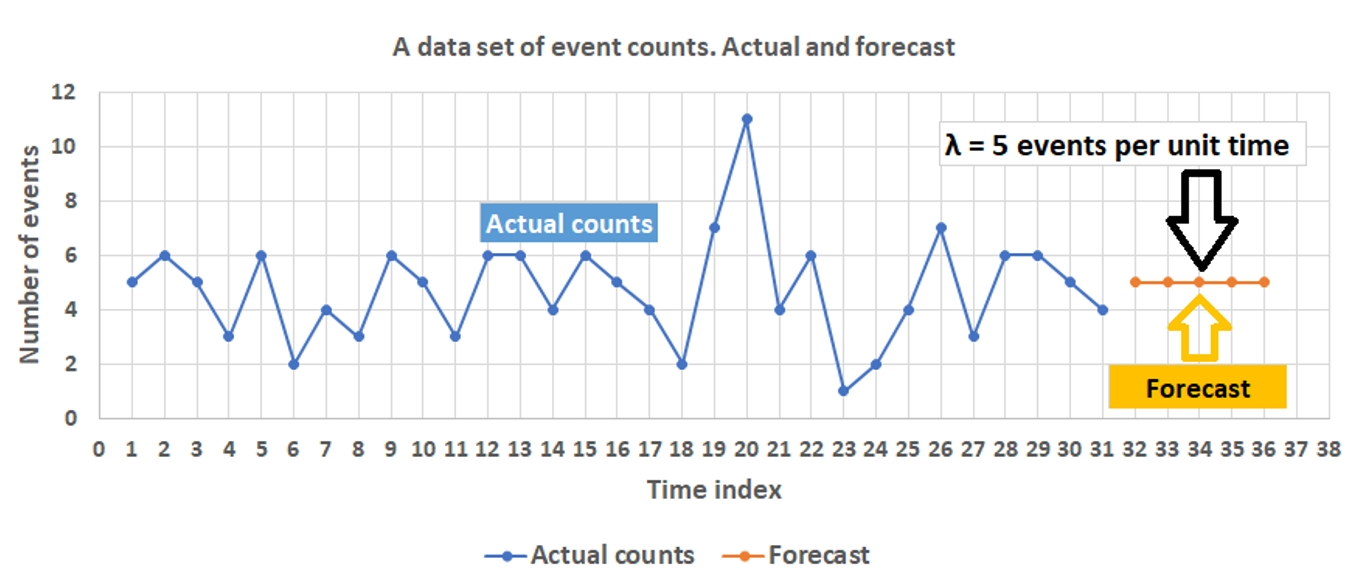
\includegraphics[width=0.8\textwidth]{pic/2.6.2.png}
    \caption{泊松回归}
\end{figure}

但实际情况中,事件发生率通常会发生变化,并不为常数。
\begin{example}
    天气条件、节假日等因素会影响骑行通过大桥的人数,即事件发生率。
\end{example}

在泊松回归中,一般选用log函数作为连接函数,即
\begin{equation}
    \ln \lambda_i =\bm{\beta}^T \mathbf{x}_i
\end{equation}
即
\begin{equation}
    \lambda_i = e^{\bm{\beta}^T \mathbf{x}_i}
\end{equation}
其中$\bm{\beta}= (\beta_1,\beta_2,\cdots,\beta_k)$为自变量$\mathbf{x}_i= (x_{i1},x_{i2},\cdots,x_{ik})$的系数向量。

似然函数,即$n$个观测的联合概率为
\begin{equation}
    L(\bm{\beta}) = \prod_{i=1}^n \frac{e^{(-e^{\bm{\beta}^T \mathbf{x}_i})}(e^{\bm{\beta}^T \mathbf{x}_i })^{y_i}}{y_i!}
\end{equation}
对数似然函数为
\begin{equation}
    \ln L(\bm{\beta}) = \sum_{i=1}^n \left(-e^{\bm{\beta}^T \mathbf{x}_i} + y_i \bm{\beta}^T \mathbf{x}_i - \ln y_i!\right)
\end{equation}

对照广义线性模型,对于泊松回归
\begin{itemize}[itemsep=0pt,parsep=0pt]
    \item 随机成分:因变量(响应变量)$Y$为服从泊松分布的随机变量,期望为$\lambda$;
    \item 系统性成分:可以包含多个解释变量,利用解释变量的线性组合来估计响应变量$Y$的期望;
    \item 连接函数:使用log函数,$\eta = g(\lambda) = \ln \lambda$。
\end{itemize}

\subsection{负二项回归(Negative Binomial Regression)}

\subsubsection{负二项分布(Negative-Binomial distribution)}

负二项分布与二项分布类似,但其描述的是在出现固定“失败”次数$r$之前,成功的次数。负二项分布的概率质量函数PMF为
\begin{equation}
    P(X=x) = \binom{x+r-1}{x}p^x(1-p)^r, x=0,1,2,\cdots
\end{equation}

但负二项分布包含两个参数,$r$和$\pi$,其期望和方差分别为
\begin{equation}
    E(X) = \frac{r(1-\pi)}{\pi} = \mu, Var(X) = \frac{r(1-\pi)}{\pi^2}
\end{equation}
负二项分布不再要求均值和方差相同,相对较弱的限制条件,也使得负二项分布可以对数据进行较好的拟合。

将发生概率$\pi$用均值$\mu$表示
\begin{equation}
    \pi = \frac{\mu}{r+\mu}
\end{equation}

负二项分布的概率质量函数PMF为
\begin{equation}
    P(Y=y_i|\mu_i,r) = \binom{y_i+r-1}{y_i}\left(\frac{\mu_i}{r+\mu_i}\right)^{y_i}\left(\frac{r}{r+\mu_i}\right)^r,y_i=0,1,2,\cdots
\end{equation}

\subsubsection{负二项回归}

在负二项回归中,一般也选用log函数作为连接函数,即
\begin{equation}
    \ln \mu_i =\bm{\beta}^T \mathbf{x}_i
\end{equation}

似然函数,即$n$个观测的联合概率为
\begin{equation}
    L(\bm{\beta}) = \prod_{i=1}^n \binom{y_i+r-1}{y_i}\left(\frac{\mu_i}{r+\mu_i}\right)^{y_i}\left(\frac{r}{r+\mu_i}\right)^r
\end{equation}
对数似然函数为
\begin{equation}
    \ln L(\bm{\beta}) = \sum_{i=1}^n \left(\ln \binom{y_i+r-1}{y_i} + y_i \ln \left(\frac{\mu_i}{r+\mu_i}\right) + r \ln \left(\frac{r}{r+\mu_i}\right)\right)
\end{equation}

对照广义线性模型,对于负二项回归
\begin{itemize}[itemsep=0pt,parsep=0pt]
    \item 随机成分:因变量(响应变量)Y为服从负二项分布的随机变量,期望为$\mu$;
    \item 系统性成分:可以包含多个解释变量,利用解释变量的线性组合来估计响应变量$Y$的期望;
    \item 连接函数:使用log函数,$\eta = g(\mu) = \ln \mu$。
\end{itemize}

\section{多目标决策}

在现实生活和实际工作中,我们遇到的问题常常会有多个目标。

\begin{example}
    综合利用水利工程的建设,通常要在适当地点修建一个水坝,并具有下述效益:

    \begin{itemize}[itemsep=0pt,parsep=0pt]
        \item 形成高水头以便发电、拦蓄洪水以防下游洪涝灾害、水库蓄水位提高后有利上游段的航运等
        \item 工程建设也要大量投资、会有淹没损失、需要安置移民
        \item 在选择水库库容(即确定坝高)的时候,就应综合考察发电、防洪、淹没(移民)、投资等多个目标
    \end{itemize}
\end{example}

多目标决策问题的特点:
\begin{itemize}[itemsep=0pt,parsep=0pt]
    \item 决策问题的目标多于一个;
    \item 多目标决策问题的目标间不可公度(Non-commensurable),即各目标没有统一的衡量标准或计量单位,因而难以进行比较。

          \begin{example}
              水利工程建设问题中的发电这一目标可以用年发电量(亿度/年)或装机容量(万千瓦)来描述,而防洪效益只能用下游免遭洪涝灾害的面积(亩)来表征。
          \end{example}
    \item 各目标间的矛盾性, 绝大部分多目标决策问题的各个备选方案在各目标之间存在某种矛盾,即如果采用一种方案去改进某一目标的值,很可能会使另一目标的值变坏。
          \begin{example}
              水利工程建设问题,想要提高发电和防洪效益,就要提高水头,增加大坝高度,但是同时也需要增加投资,加大淹没损失和移民数量
          \end{example}
\end{itemize}

\subsection{多目标优化问题(Multi-Objective Optimization Problems, MOOP)}

实际生活中面临的决策问题,往往涉及多个目标。

这些目标之间通常是相互矛盾的( conflicting objectives ) , 我们需要在不同的目标之间进行权衡, 从而做出最终的决策。

如果所面对的决策问题, 虽然具有多个目标, 但是目标之间不存在矛盾竞争关系,那么我们可以称之为退化的多目标优化问题。 在此情况下, 不同目标可以同时达到最优解, 因此, 不需要将其转化为多目标优化问题进行求解。

\textbf{多目标优化问题(Multi-Objective Optimization Problems, MOOP)}:

\begin{itemize}[itemsep=0pt,parsep=0pt]
    \item 多目标优化需要同时优化两个或者两个以上的目标函数,且不能显式地平衡它们,即不存在同时优化每个目标函数的解;
    \item 多目标优化的结果是一组解集(set of solutions), 其中的每个解都是在不同目标之间折衷的结果,每个解相对其他解都有其独特的优势。
\end{itemize}

多目标优化问题的数学表达
\begin{equation}
    \begin{aligned}
         & \min_{x \in X} f(x) = (f_1(x),f_2(x),\cdots,f_m(x)) \\
         & s.t.   \begin{cases}
                      \quad x \in X                   \\
                      g_j(x) \leq 0, j = 1,2,\cdots,J \\
                      h_k(x) = 0, k = 1,2,\cdots,K
                  \end{cases}
    \end{aligned}
\end{equation}
多目标优化问题的三要素:决策变量$x$、目标函数$f(x)$、约束条件$g_j(x) \leq 0, j = 1,2,\cdots,J$和$h_k(x) = 0, k = 1,2,\cdots,K$。

决策变量: $x=(x_1, x_2, \cdot, x_N)^T$ 是$N$维决策变量,决策变量是可以被认为控制的,并能对指标属性产生影响, 决策变量的不同取值对应不同决策方案;

目标函数: 是决策指标的数学表达,为连续函数。决策者希望所有指标同时达到最优,但在现实中一般无法满足。所有目标函数构成了多目标优化问题的目标函数集合(向量)。

约束条件: 为决策变量需要满足的限制条件,使用还有等式和不等式的约束函数来表示, 满足所有所有约束条件的一组决策变量可以称之为一个“可行解” ,多目标优化问题中所有可行解构成了整个可行域。

\begin{figure}[ht]
    \centering
    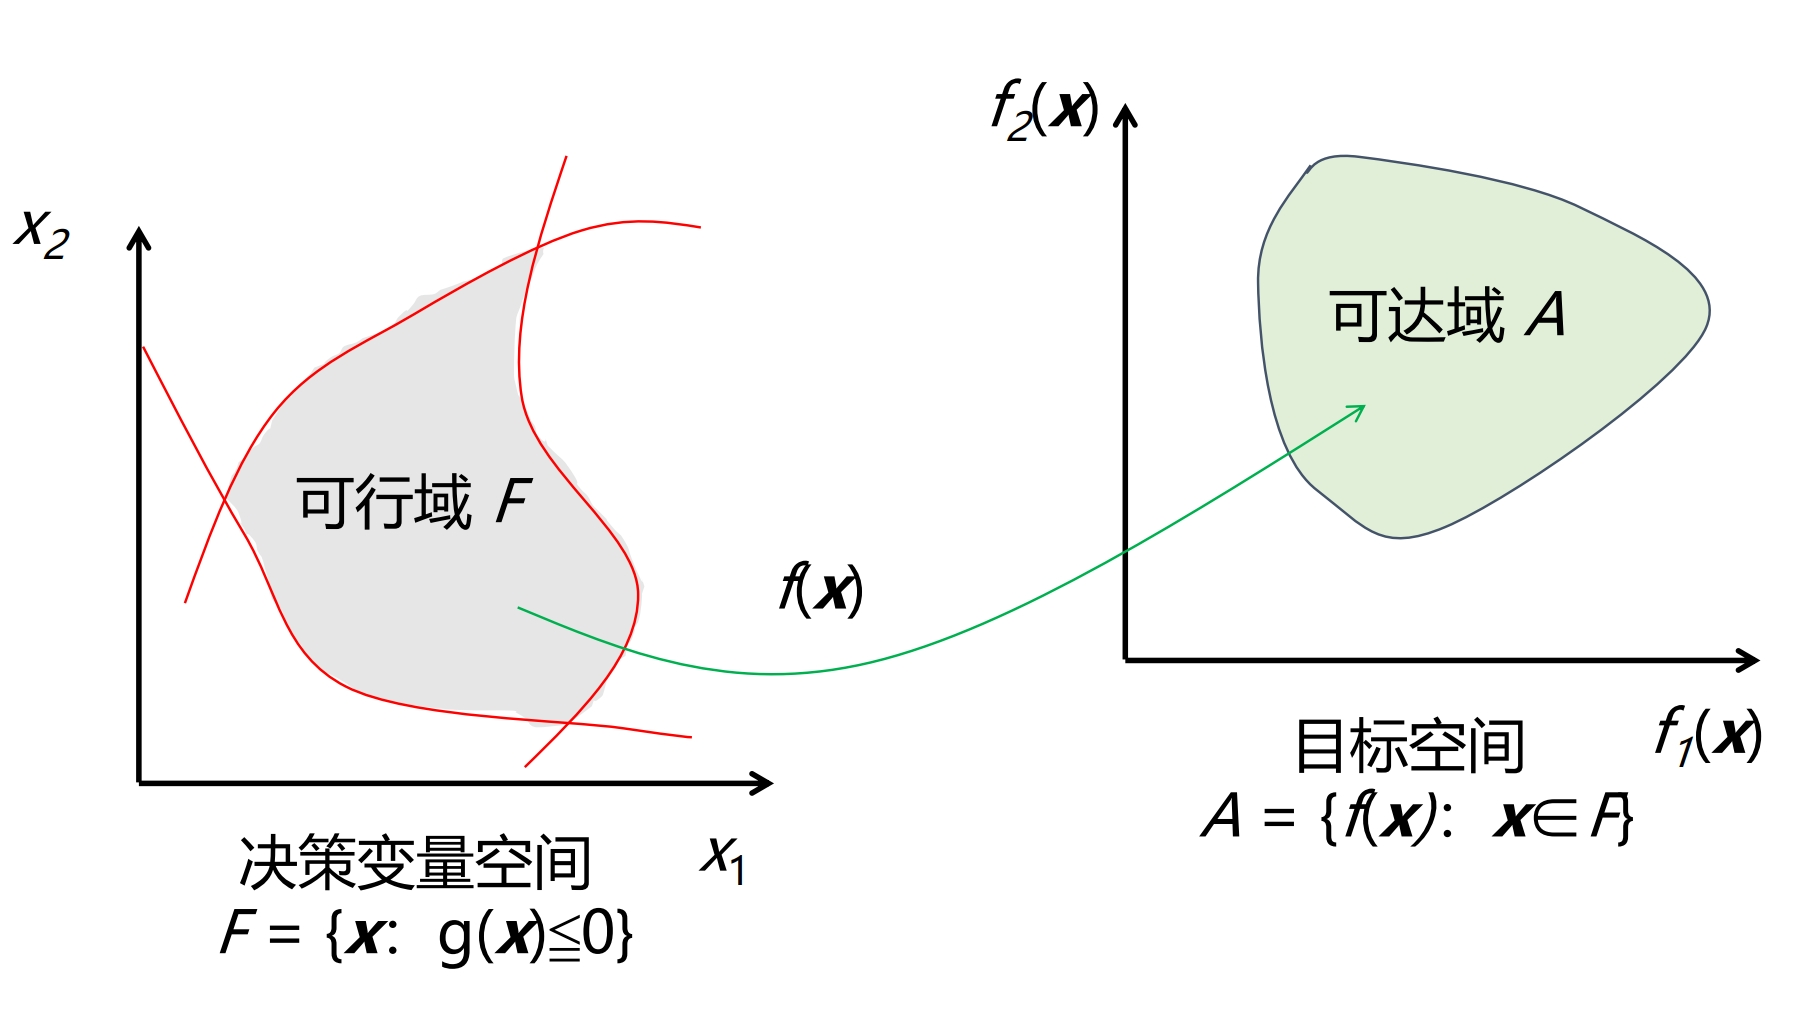
\includegraphics[width=0.8\textwidth]{pic/2.7.1.png}
    \caption{多目标优化问题}
\end{figure}

\subsection{占优性(Dominance)}

在单目标优化问题中,通过比较目标函数值可以确定一种决策方案是否比另一种方案优越,因此最优解只有一个,然而

\begin{itemize}[itemsep=0pt,parsep=0pt]
    \item 多目标优化问题中,目标函数集合组成一个向量,各目标之间相互制约,试图改善一个目标往往以损失其他目标为代价, 无法直接比较不同方案之间的优劣。
    \item 多目标优化问题中,一般采用占优性(Dominance) 的概念来衡量一组解的适用性。
\end{itemize}

\subsubsection{占优性检验}

可行域中的两个决策向量$a, b \in X$ , $a$占优(dominates) $b$,当且仅当$a$的所有目标函数都不劣于对应的$b$的目标函数,$a$至少有一个目标函数严格优于对应的$b$的目标函数。

数学描述为
\begin{equation}
    a \succ b \Leftrightarrow \forall i \in \{1,2,\cdots,m\}, f_i(a) \leq f_i(b) \land \exists i \in \{1,2,\cdots,m\}, f_i(a) < f_i(b)
\end{equation}

\subsubsection{帕累托最优解( Pareto Optimal Solution)}

帕累托最优解( Pareto Optimal Solution): 如果存在某个决策向量,在整个可行域中,不存在任何决策向量占优该决策向量,则称该决策向量为帕累托最优解( Pareto Optimal Solution), 或被称为非支配解(Non-dominated Solution), 或者非劣解(Non-inferior Solution)。

帕累托最优解集合(Pareto Optimal Set): 可行域中所有帕累托最优解组成的集合。

帕累托前缘( Pareto Front): 所有帕累托最优解对应的目标函数构成了多目标优化问题的帕累托前缘(Pareto Front),即将帕累托最优解集合投射到目标函数空间,所组成的边界。

目标最优问题的目标是寻找所有逼近帕累托前缘的解,即寻找所有帕累托最优解。

\begin{figure}[ht]
    \centering
    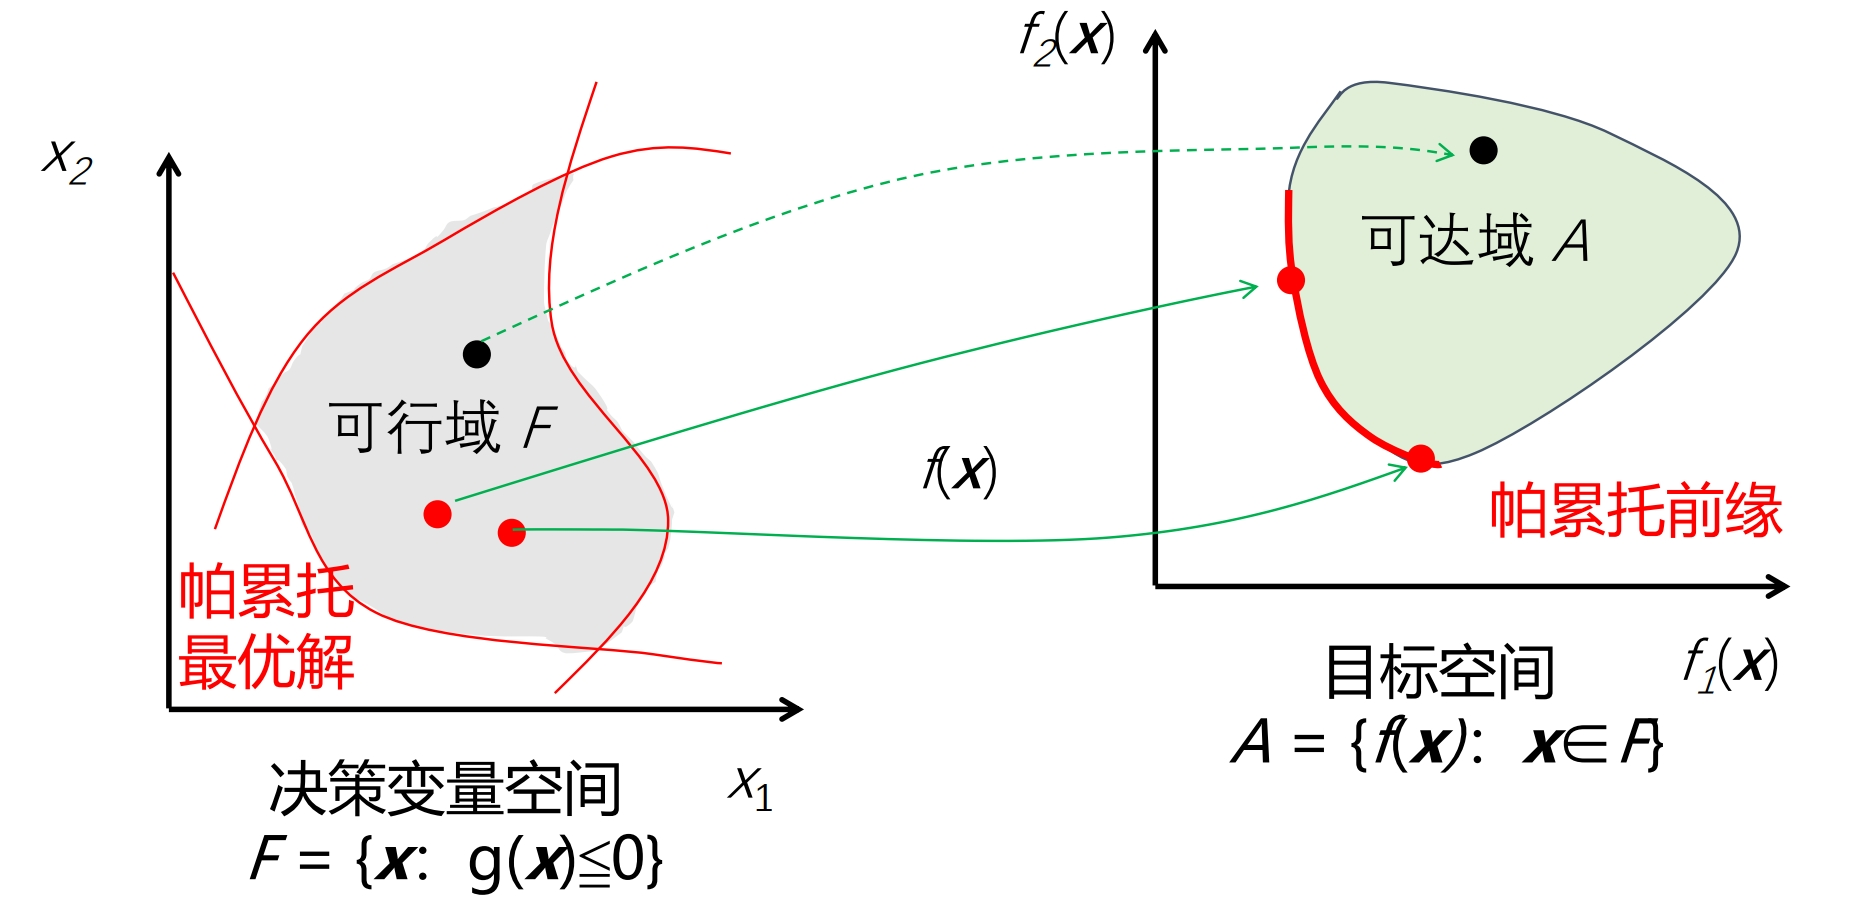
\includegraphics[width=0.8\textwidth]{pic/2.7.2.png}
    \caption{帕累托最优解}
\end{figure}

\subsection{多目标最优问题的求解方法}

标量化求解策略(Scalarization):将多目标优化问题转化为一组单目标优化问题
\begin{itemize}[itemsep=0pt,parsep=0pt]
    \item 加权求和法(weighted sum)
    \item epsilon约束求解方法(epsilon-constraint)
    \item Compromise programming
\end{itemize}

参数化搜索(Parametric sweep) :利用一组参数$\{p_1, p_2, \cdots, p_{N_p}\}$,每一个参数都将多目标问题转化为唯一的单目标优化子问题,可以寻找到帕累托前缘( ParetoFront) 上的$N_p$个点。

\begin{figure}[ht]
    \centering
    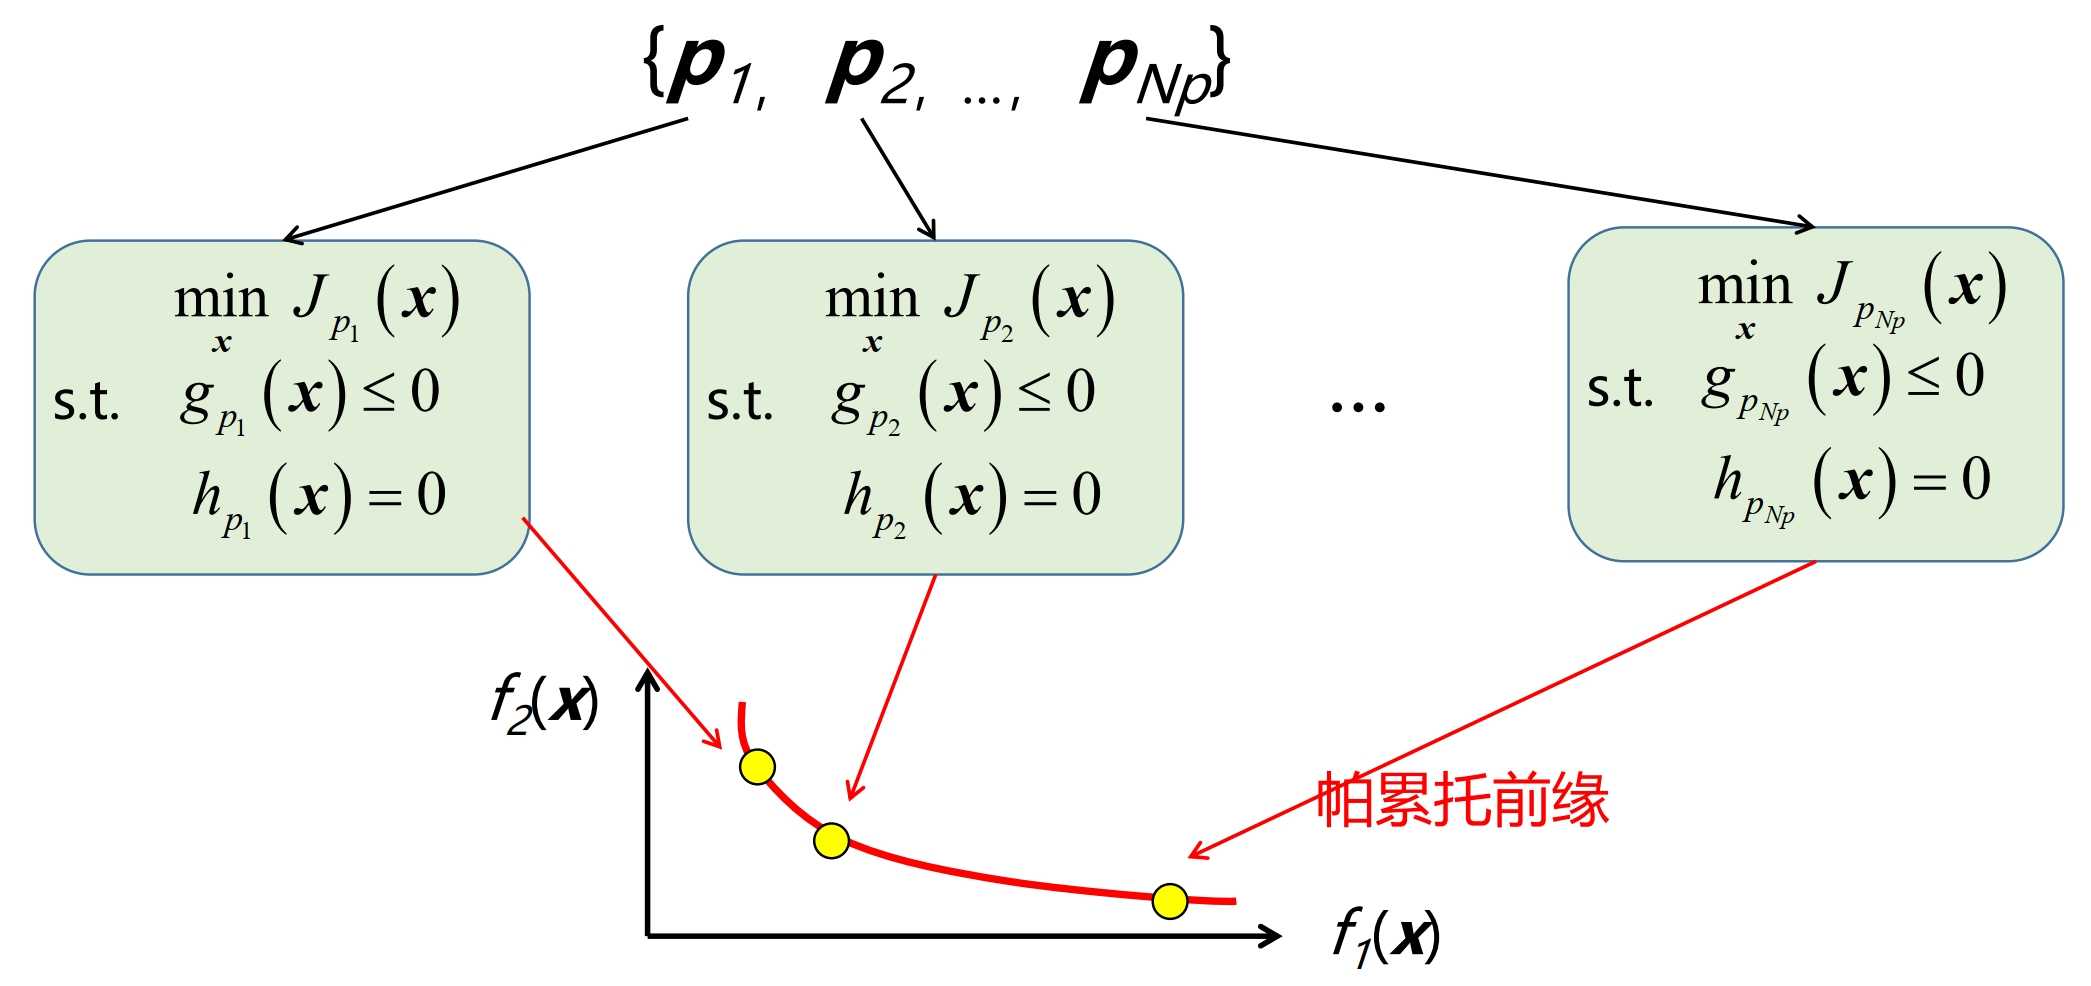
\includegraphics[width=0.8\textwidth]{pic/2.7.3.png}
    \caption{多目标最优问题的求解方法}
\end{figure}

\subsubsection{加权求和法(weighted sum)}

通过各个目标函数的线性组合来构建一个集成的新目标函数$J(x)$,因此也被称为线性加权求和法,是最基础和简单的标量化方法。

每一种权重$w$对应一组具有相同斜率的平行线,代表新目标函数的等值线
\begin{equation}
    J(x) = \sum_{i=1}^m w_i f_i(x)
\end{equation}

\begin{figure}[ht]
    \centering
    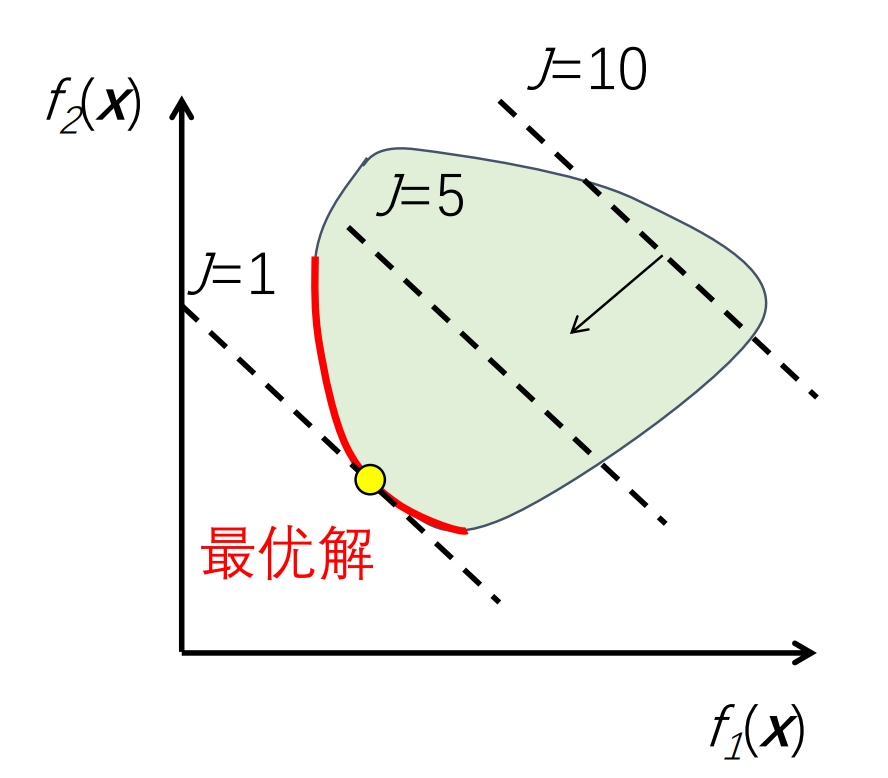
\includegraphics[width=0.4\textwidth]{pic/2.7.4.png}
    \caption{加权求和法}
\end{figure}

对于权重,通常采用归一化策略,即
\begin{equation}
    \sum_{i=1}^m w_i = 1 , 0 \leq w_i \leq 1
\end{equation}

这里的权重组合就是之前提到的变换参数$p$
\begin{equation}
    w = (w_1, w_2, \cdots, w_m)^T
\end{equation}
使用不同权重组合,构成新的单目标最优化子问题,通过最优化子问题,获得帕累托前缘上不同的点。

\begin{example}
    以双目标问题为例

    当使用加权求和方法时,如果将目标函数$f_1(x)$的权重设为$0$,$f_2(x)$的权重即为$1$。此时,获得的帕累托前缘上的点($M_2$)被称为一个锚点(anchor point)。
    \begin{figure}[ht]
        \centering
        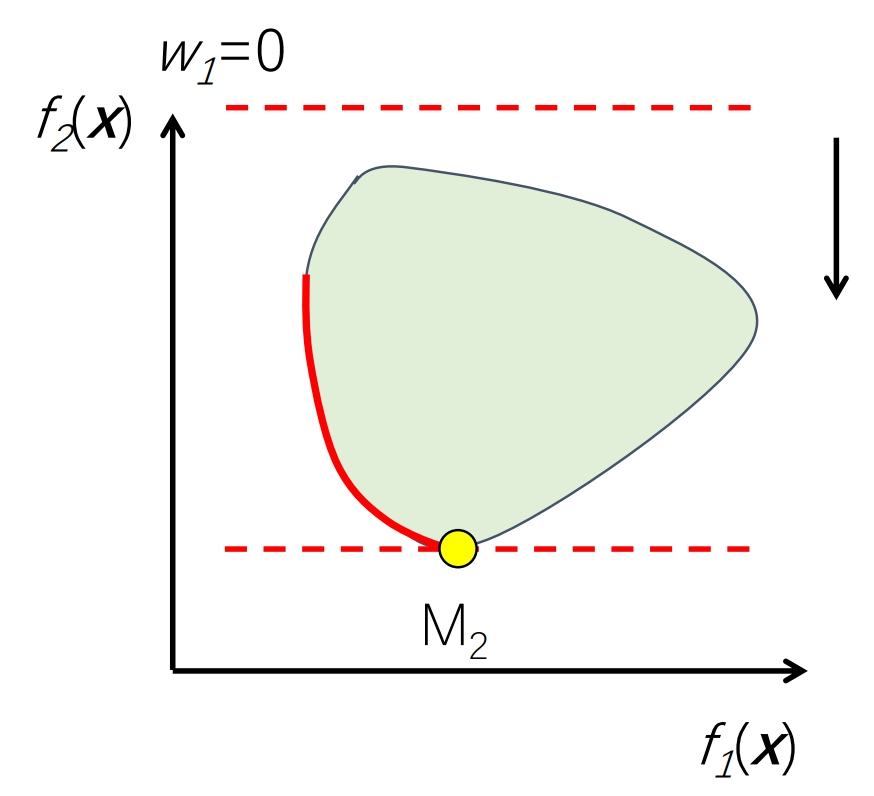
\includegraphics[width=0.3\textwidth]{pic/2.7.5.png}
        \caption{加权求和法——锚点}
    \end{figure}

    当使用加权求和方法时,如果将目标函数$f_1(x)$的权重设为$1$,$f_2(x)$的权重即为$0$。此时,获得的帕累托前缘上的点($M_1$)被称为另一个锚点。
    \begin{figure}[ht]
        \centering
        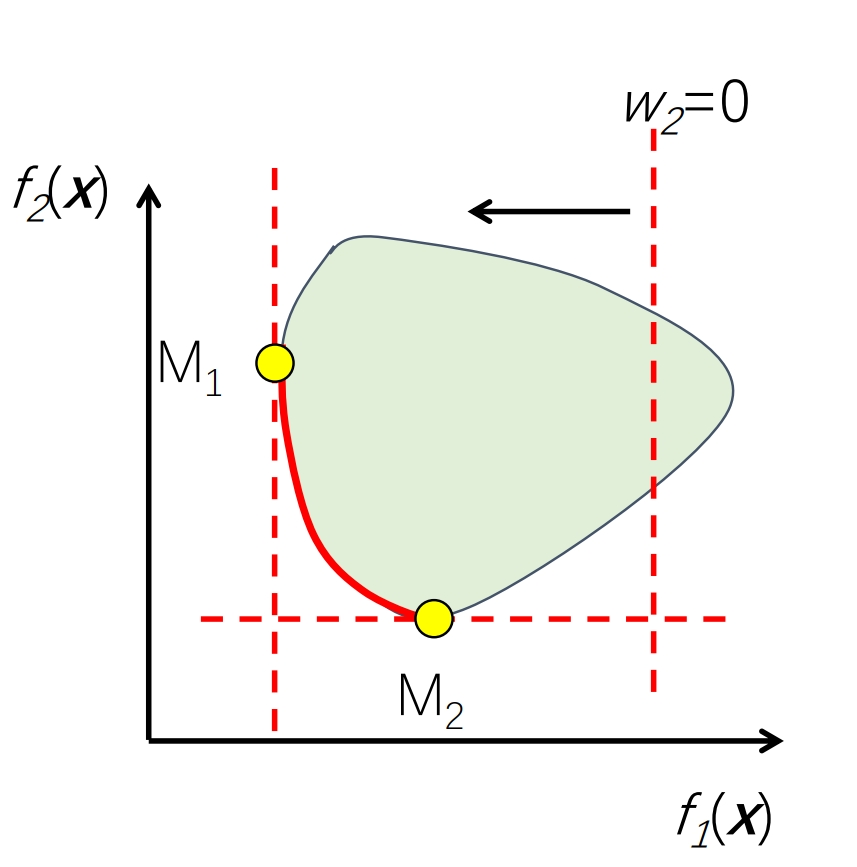
\includegraphics[width=0.3\textwidth]{pic/2.7.6.png}
        \caption{加权求和法——锚点}
    \end{figure}

    这两条线的交点被称为理想点(Utopia point)
    \begin{figure}[ht]
        \centering
        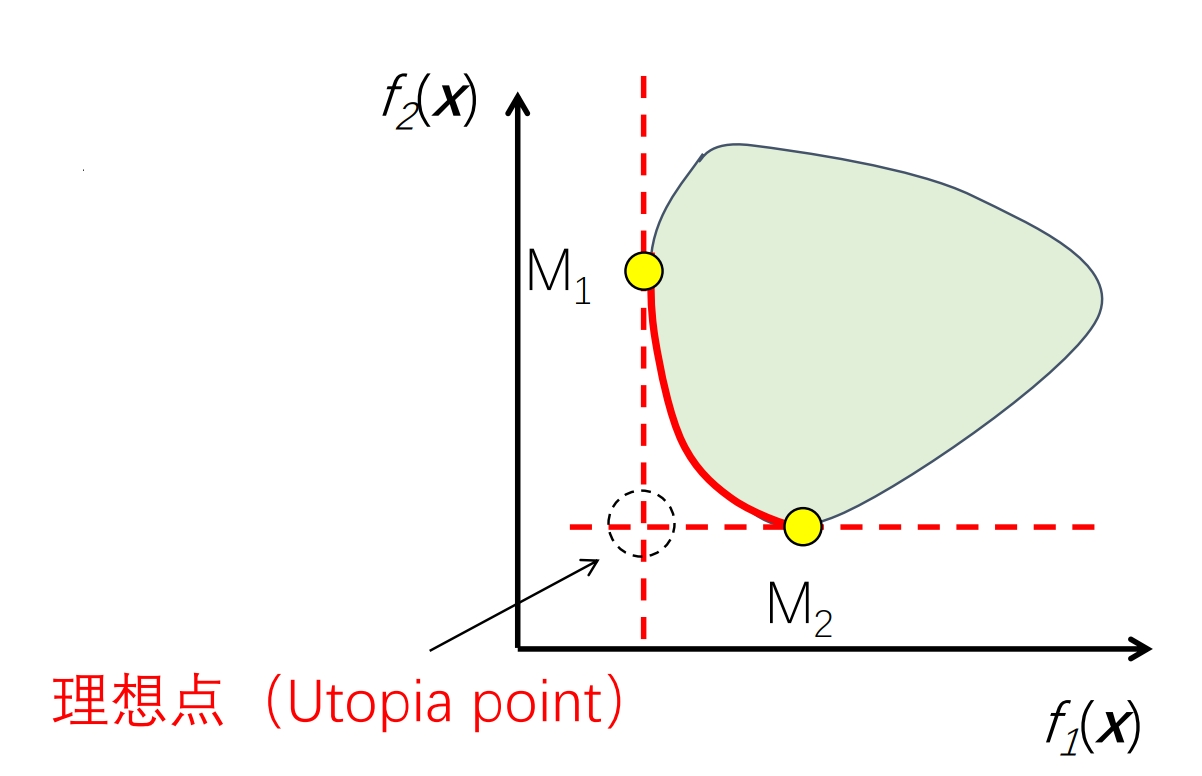
\includegraphics[width=0.3\textwidth]{pic/2.7.7.png}
        \caption{加权求和法——理想点}
    \end{figure}

    该点可使目标函数同时达到最优解,但是该点一般不在可达域内,即在可行域内,不存在这样的点,通过目标函数投影后位于理想点位置。
    ⚫
    对于退化多目标优化问题,目标函数可以同时达到最优, 此时理想点存在,但是退化多目标优化问题一般不需要采用复杂求解方法。

    对于其他任意的权重组合$w_i$, 产生的帕累托前缘上的点都位于锚点$M_1$与$M_2$之间
    \begin{figure}[ht]
        \centering
        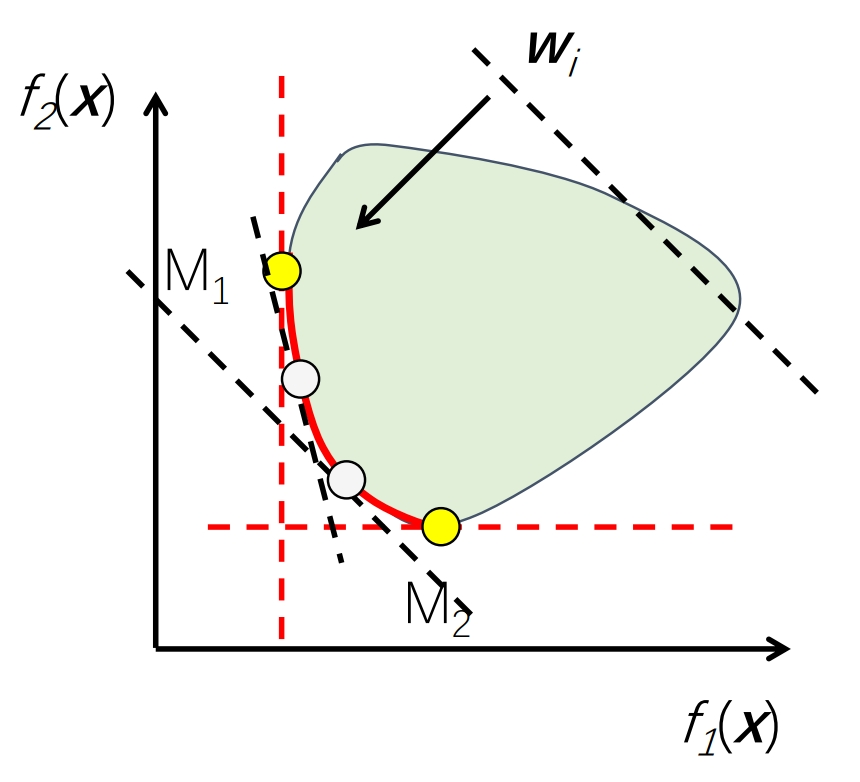
\includegraphics[width=0.3\textwidth]{pic/2.7.8.png}
        \caption{加权求和法——帕累托前缘}
    \end{figure}

    通过系统化地改变权重组合可以获得帕累托前缘上的多个点.
\end{example}

加权求和法优势
\begin{itemize}[itemsep=0pt,parsep=0pt]
    \item 概念上简单, 容易理解;
    \item 构建方式简单, 保持线性,易于实现。
\end{itemize}

加权求和法缺点
\begin{itemize}[itemsep=0pt,parsep=0pt]
    \item 目标函数空间中,获得的帕累托前缘上的点分布可能不均匀;
    \item 无法获得非凸区域(non-convex regions) 的帕累托非支配点(帕累托前缘)。
\end{itemize}

\subsubsection{epsilon约束求解方法(epsilon-constraint)}

epsilon约束求解方法: 仅保留一个多目标优化问题中的目标函数构成单目标优化问题,将其他目标函数转化为具有边界的约束条件。

\begin{equation}
    \begin{aligned}
         & \min_{x \in X} f_n(x)                                    \\
         & s.t.   \begin{cases}
                      \quad x \in X                   \\
                      g_j(x) \leq 0, j = 1,2,\cdots,J \\
                      h_k(x) = 0, k = 1,2,\cdots,K    \\
                      f_i(x) \leq \epsilon_i, i = 1,2,\cdots,M, i \neq n
                  \end{cases}
    \end{aligned}
\end{equation}

\begin{example}
    以双目标问题为例

    \begin{equation}
        \begin{aligned}
             & \min_{x \in X} f_1(x)                                                            \\
             & s.t.   \begin{cases}
                          \quad x \in X                   \\
                          g_j(x) \leq 0, j = 1,2,\cdots,J \\
                          f_2(x) \leq \epsilon_i , \epsilon_1 < \epsilon_2 < \cdots < \epsilon_{N_p}
                      \end{cases}
        \end{aligned}
    \end{equation}

    求解第一个单目标最优化子问题
    \begin{equation}
        \begin{aligned}
             & \min_{x \in X} f_1(x)        \\
             & s.t.   \begin{cases}
                          \quad x \in X \\
                          g(x) \leq 0   \\
                          f_2(x) \leq \epsilon_1
                      \end{cases}
        \end{aligned}
    \end{equation}
    如图,获得帕累托前缘上的点$M_1$
    \begin{figure}[ht]
        \centering
        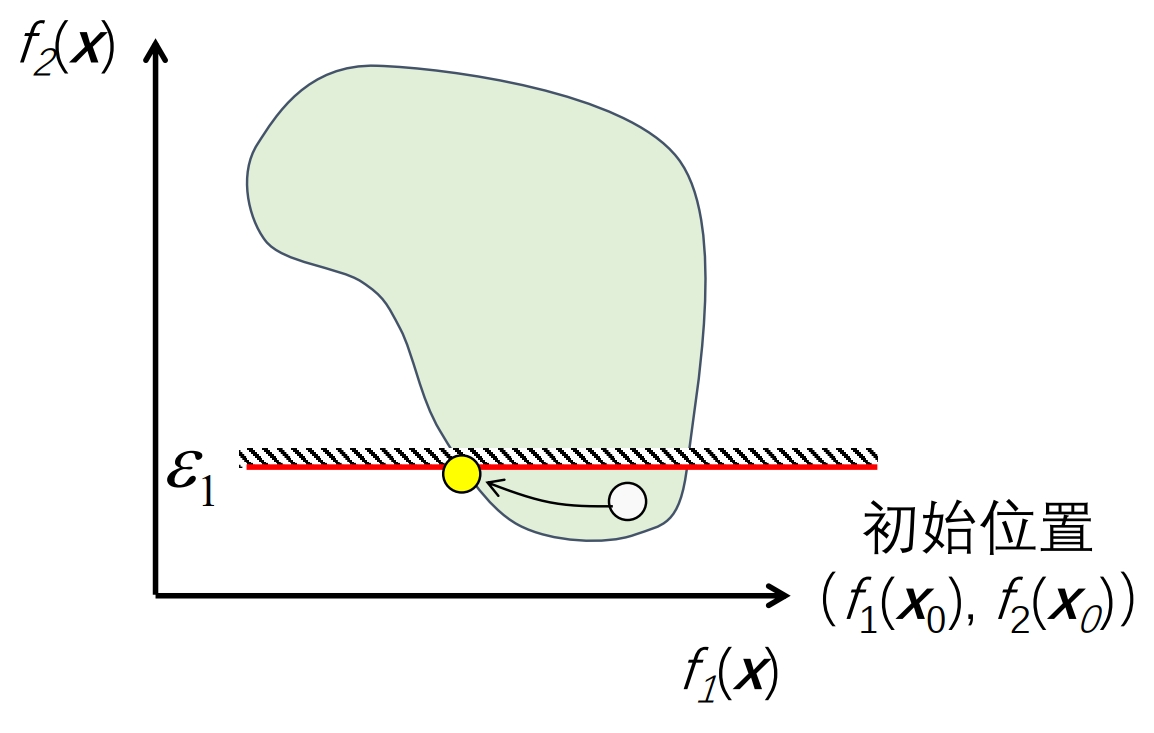
\includegraphics[width=0.3\textwidth]{pic/2.7.9.png}
        \caption{epsilon约束求解方法——帕累托前缘}
    \end{figure}

    同理
    \begin{equation}
        \begin{aligned}
             & \min_{x \in X} f_1(x)        \\
             & s.t.   \begin{cases}
                          \quad x \in X \\
                          g(x) \leq 0   \\
                          f_2(x) \leq \epsilon_2
                      \end{cases}
        \end{aligned}
    \end{equation}
    得到帕累托前缘上的点$M_2$
    \begin{figure}[ht]
        \centering
        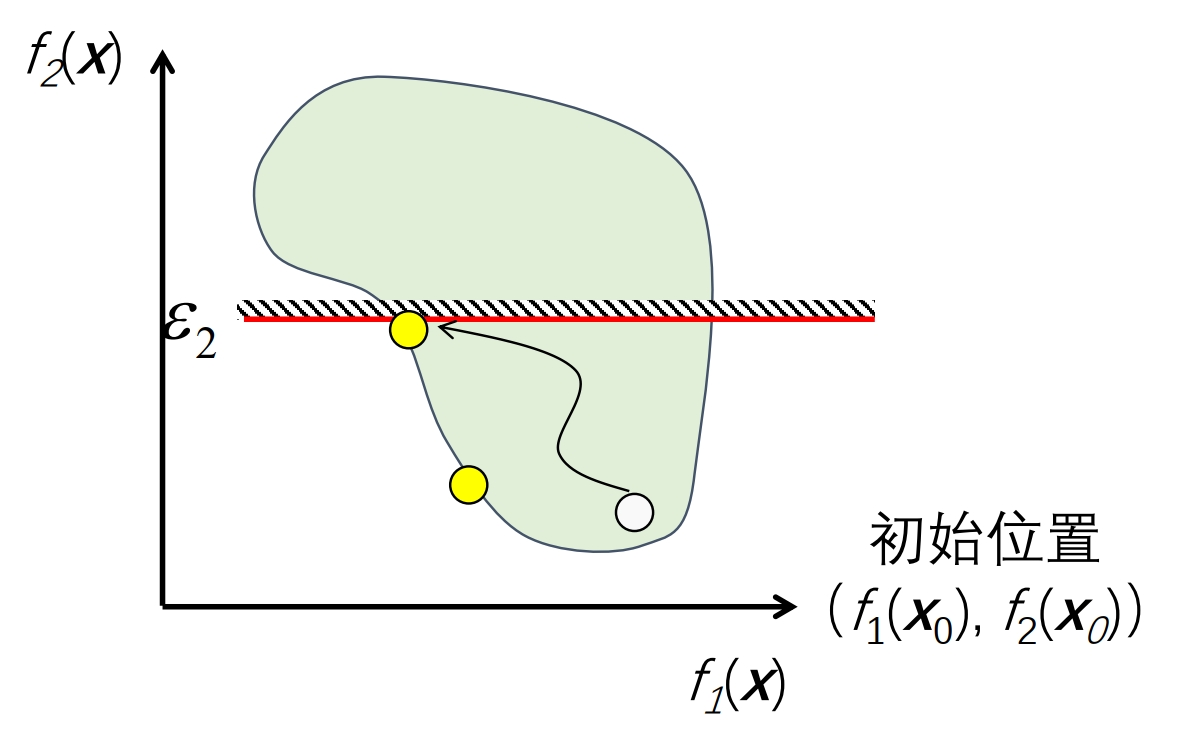
\includegraphics[width=0.3\textwidth]{pic/2.7.10.png}
        \caption{epsilon约束求解方法——帕累托前缘}
    \end{figure}
    以此类推。
\end{example}

epsilon约束求解方法:仅保留一个多目标优化问题中的目标函数构成单目标优化问题,将其他目标函数转化为具有边界的约束条件。

通过系统性地改变约束条件的边界,生成帕累托前缘。

与加权求和法不同, epsilon约束求解方法不是一种集成目标函数方法,因为只保留一个目标函数,并没有对多目标函数进行组合。

epsilon约束求解方法优势
\begin{itemize}[itemsep=0pt,parsep=0pt]
    \item 可以较为可靠地获得非凸区域的帕累托前缘;
    \item  在目标函数空间中,可以产生较为均与的非支配点,构成帕累托前缘;
    \item 保持求解问题的线性性。
\end{itemize}

% \chapter{数据与智能决策}

\section{人工智能决策}

人工智能:机器学习/构建数据特征与预期指标的关系


\end{document}